%/**
% * @file tese.tex
% * @brief This file have the configuration parameters of Dr. Degree thesis.
% * @ingroup Documentation
% * @author $Author: rodcosta $
% * @date $Date: 2009/07/12 18:54:10 $
%**
\documentclass[12pt,a4paper,oneside,final]{book}
%%% para vers\~{o}es parciais do dumento final utilizar:
%\documentclass[12pt,a4paper,draft]{book}
%\documentclass[12pt,a4paper,twoside,fleqn,draft]{book}
%%%%%%%%%%%%%%%%%%%%%%%%%%%%%%%%%%%%%%%%%%%%%%%%%%%%%%%%%%%%%%%%
%%% PREAMBULO DO DOCUMENTO COME\c{C}A AQUI
%\usepackage{natbib}
%\bibliographystyle{elsart-harv}
%inclui coisas da abnt
%\bibliographystyle{abntcite}
%\usepackage{hvfoat}
\usepackage{datetimepor}
\usepackage{monografia}
\usepackage{multicol}
\usepackage{rotating}
\usepackage{monografia_defs}
\usepackage[none]{hyphenat}
% Permite utilizar configuracoes da linguagem portugesa do Brasil e Inglesa
\usepackage[english,brazil]{babel}
% Permite especificar codificacao das entradas (caracteres acentuados - � - sem usar \'a)
\usepackage[latin1]{inputenc}
\usepackage{assinatura}
\usepackage{color}
\usepackage{multirow}
% \bibstyle{abnt-alf}
\usepackage{sidecap}
\usepackage{ifthen}
\usepackage{psfrag}
\usepackage{supertabular}


%
\newcommand{\titulo}{MDiag: Ferramenta de Diagn�stico de Falhas em Mem�ria para Sistemas Operacionais Linux.}
\newcommand{\autor}{Francisco Pl�nio Oliveira Silveira}
\newcommand{\orientador}{Prof. Msc. Alexandre Augusto da Penha Coelho}
\newcommand{\coorientador}{Prof. Dr. Helano de Sousa Castro}
\newcommand{\membroa}{Prof. Dr. Jos\'{e} Marques Soares}
\newcommand{\membrob}{Prof. Msc. Rodrigo Carvalho Souza Costa}
\renewcommand{\eqref}[1]{equa\c{c}\~{a}o~\ref{#1}}
\newcommand{\eqrefp}[1]{equa\c{c}\~{o}es~\ref{#1}}
\newcommand{\ok}{$\blacksquare$}
\newcommand{\nok}{$\square$}

\newcommand{\secao}{\section}
\newcommand{\capitulo}{\chapter}
\newcommand{\subsecao}{\subsection}

\newcommand{\secref}[1]{se\c{c}\~{a}o~\ref{#1}}
\newcommand{\secrefp}[1]{se\c{c}\~{o}es~\ref{#1}}
\newcommand{\tabref}[1]{Tabela~\ref{#1}}
\newcommand{\tabrefp}[1]{Tabelas~\ref{#1}}
\newcommand{\figref}[1]{Figura~\ref{#1}}
\newcommand{\figrefp}[1]{Figuras~\ref{#1}}

\usepackage[breaklinks,final,pdftitle={\titulo},pdfauthor = {\autor}]{hyperref}

%\usepackage{hyperref}
\usepackage[sort]{cite}
\usepackage[alf,abnt-and-type=e,abnt-full-initials=no,abnt-last-names=abnt,abnt-etal-list=2,abnt-etal-text = emph]{abntcite}
\newcommand{\citet}[1]{\citeonline{#1}}

%\newcommand{\eqref}[1]{(\ref{#1})}
\newcolumntype{Y}{>{\centering\arraybackslash}X}
%\newcommand{\secref}[1]{se\c{c}\~{a}o~\ref{#1}}
%\newcommand{\secrefp}[1]{se\c{c}\~{o}es~\ref{#1}}
%\newcommand{\tabref}[1]{Tabela~\ref{#1}}
%\newcommand{\tabrefp}[1]{Tabelas~\ref{#1}}
%\newcommand{\figref}[1]{Figura~\ref{#1}}
%\newcommand{\figrefp}[1]{Figuras~\ref{#1}}
%
%\usepackage[dvips]{graphicx}
%\usepackage[portuges]{babel}
\usepackage[printonlyused]{acronym}
\usepackage{hvfloat}
\usepackage{longtable}
\usepackage{supertabular}
\usepackage{tabularx}
\usepackage{here}
%\usepackage{abntcite}
\begin{document}
%padronizacao
\DeclareGraphicsExtensions{.jpg,.pdf,.mps,.png}

%\usepackage[final]{pdfpages}
%\usepackage{Fancyhdr}
%\bibliographystyle{IEEEtranPor}
% \includeonly{capa,agradecimentos}
% \includeonly{capa_externa,capa}
%%% PREAMBULO DO DOCUMENTO ACABA AQUI
%%%%%%%%%%%%%%%%%%%%%%%%%%%%%%%%%%%%%%%%%%%%%%%%%%%%%%%%%%%%%%%%

%%%%%%%%%%%%%%%%%%%%%%%%%%%%%%%%%%%%%%%%%%%%%%%%%%%%%%%%%%%%%%%%
%%% CAPA

\pagenumbering{Roman}
\thispagestyle{empty}%

\begin{center}
    
\includegraphics[width=2.5cm,bb=0 0 382 465]{figs/ufc.jpg} \\%
    \textsc{
    Universidade Federal do Cear\'{a} \\%
    Departamento de Engenharia de Teleinform\'{a}tica \\%
    Programa de P\'{o}s Gradua\c{c}\~{a}o em Engenharia de Teleinform\'{a}tica\\
    }
    \vspace{2.5 cm}%
%   {\normalsize    \textbf{Autor} \\%
%                     \textbf{Carlos H\'{e}racles Morais de Lima}} \\%
    {                \textbf{\autor}
    } \\%

    \null\vfill%%
    \vspace{.2cm}%
%        \textbf{Proposta de Tese submetida a Coordena\c{c}\~{a}o do Programa de P\'{o}s Gradua\c{c}\~{a}o em Engenharia de Teleinform\'{a}tica}\\
        {\Large         \textbf{\titulo}\\}



    \null\vfill%%
    \vspace{1 cm}%
    {\normalsize    \textsc{Fortaleza -- Cear\'{a} \\%
                            \monthname~2011 }}
\end{center}

\thispagestyle{empty}%

\begin{center}
    %
\includegraphics[width=2.5cm]{figs/ufc.jpg} \\%
%    \textsc{
%    Universidade Federal do Cear\'{a} \\%
%    Departamento de Engenharia de El\'{e}trica \\%
%    Programa de P\'{o}s Gradua\c{c}\~{a}o em Engenharia de Teleinform\'{a}tica\\
%    }
    \null\vfill%%
    \vspace{.25cm}%
    {\normalsize    \textbf{Autor:} \\%
                    \upshape{\autor}
                    }\\%

    \null\vfill%%
    \vspace{.25cm}%
    {\normalsize    \textbf{Orientador:} \\%
                    \upshape{\orientador}
                    } \\%
    \null\vfill%%
    \vspace{.25cm}%
%    {\normalsize    \textbf{Co-orientador:} \\%
%                    \upshape{\coorientador}
%                    } \\%

%    \null\vfill%%
    \vspace{.25cm}%
    {\large         \titulo\\}

    \null\vfill%%
    \vspace{.25cm}%
    \begin{tabularx}{\textwidth}{XX}

    \null\vfill \\
    &
    Monografia de Conclus\~{a}o de Curso apresentada \`{a} Coordena\c{c}\~{a}o do Curso de Gradua\c{c}\~{a}o em Engenharia de Teleinform\'{a}tica da Universidade Federal do Cear\'{a} como parte dos requisitos para obten\c{c}\~{a}o do grau de \textbf{Engenheiro de Teleinform\'{a}tica}. \\

    \end{tabularx}

    \null\vfill%%
    \vspace{.25cm}%

    {\normalsize    \textsc{Fortaleza -- Cear\'{a} \\%
                            \monthname~\the\year}}
\end{center}

%\thispagestyle{empty}%

\begin{center}
    %\includegraphics[width=2.5cm]{figs/UFC.eps} \\%
    \textsc{ \autor } \\
     \vspace{.5 cm} \textbf{ \titulo }     \\
\end{center}
    \vspace{.2 cm}
    Esta Tese foi julgada adequada para a obten\c{c}\~{a}o dos cr\'{e}ditos da disciplina Qualifica\c{c}\~{a}o de Doutorado II e aprovada em sua forma final pelo programa de P\'{o}s Gradua\c{c}\~{a}o em Engenharia de Teleinform\'{a}tica da Universidade Federal do Cear\'{a}.
    \assinatura{\autor}
    \vspace{0.2 cm}
     Banca Examinadora:
     \assinatura{\orientador \\ Orientador}
     \assinatura{\membroa}
     \assinatura{\membrob}
     \assinatura{\membroc}
     \assinatura{\membrod}
     \vspace{0.2 cm}%\null\vfill%%

\begin{center}
    {\normalsize    Fortaleza, \today}
\end{center}

\frontmatter \pagestyle{roman}
%%%%%%%%%%%%%%%%%%%%%%%%%%%%%%%%%%%%%%%%%%%%%%%%%%%%%%%%%%%%%%%%
%%% RESUMO

\pdfbookmark[1]{Resumo}{CHP:RESUM0}
\chapter*{Resumo}
\label{CHP:RESUM0}
\thispagestyle{empty}
\acresetall
\PARstartOne{O}{s} sistemas de diagn�stico de falhas v�m adquirindo import�ncia na computa��o devido � complexidade dos dispositivos digitais. Seu uso na identifica��o de problemas de \emph{hardware} tem se tornado uma demanda crescente tanto para empresas especializadas em computadores, como montadoras e fabricantes e mesmo para usu�rios dom�sticos, que desejam verificar a integridade do seu equipamento.

Neste trabalho, foi desenvolvida uma ferramenta de diagn�stico de falhas em mem�rias, chamada MDiag. O \emph{software} foi constru�do como uma aplica��o para sistemas operacionais Linux. Todo o projeto e implementa��o foi embasado por um amplo estudo sobre falhas em mem�rias, algoritmos de detec��o de falhas em mem�rias e o controle deste componente atrav�s do Linux.

Tamb�m foi desenvolvido um sistema autom�tico de gera��o e inser��o de falhas, utilizando funcionalidades de \emph{debug} presentes na maioria dos processadores atuais. Este sistema foi usado para testar e validar o MDiag quanto a cobertura de falhas.

Foram realizados testes reais com placas de mem�rias defeituosas, onde os resultados do MDiag foram comparados com os de ferramentas utilizadas no mercado.
\newline

\noindent \textbf{Palavras-chaves:} Modelagem, Teste, Algoritmo, Cobertura, Complexidade, LinuxMM.

\chapter*{Abstract}
\label{CHP:ABSTRACT}%%
\thispagestyle{empty}

%\PARstartOne{O}{s} sistemas de diagn�stico de falhas v�m adiquirindo import�ncia na computa��o devido � complexidade dos dispositivos digitais. Seu uso na identifica��o de problemas de \emph{hardware} tem se tornado uma demanda crescente tanto para empresas especializadas em computadores, como montadoras e fabricantes, quanto para usu�rios dom�sticos que desejam verificar a integridade do seu equipamento.

\PARstartOne{F}{ault} diagnosis systems has growing in importance on the computing due to the complexity of the digital devices. Its use to identiying hardware's malfunction has become an ascenceding demand for both, companies specialized in computers, such as assemblers and manufacturers, as well as for home users who want to check the integrity of your equipment.

%Neste tabalho, foi desenvolvida uma ferramenta de diagn�stico de falhas em mem�rias, chamada MDiag. O \emph{software} foi constru�do como uma aplica��o para sistemas operacionais Linux. Todo o projeto e implementa��o foi embasado por um amplo estudo sobre falhas em mem�rias, algitmos de detec��o de falhas em mem�rias e o controle deste componente atrav�s do Linux.

In this study, we developed a tool for fault diagnosis in memories, called MDiag. It was built as an application for Linux operating systems. All the design and implementation was based on an extensive study of memory faults, fault detection algorithms and Linux memory menagement.

%Tamb�m foi desenvolvido um sistema autom�tico de gera��o e inser��o de falhas utilizando funcionalidades de \emph{debug} presentes na maioria dos processadores atuais. Este sistema foi usado para testar e validar o MDiag quanto a cobertura de falhas.

It was also developed an automatic system for fault generation and insertion using debug features available in most of current processors. This system was used to test and validate the MDiag as its fault coverage.

%Foram realizados testes reais com placas de mem�rias defeituosas, onde os resultados do MDiag foram comparados com os de ferramentas utilizadas no mercado.

Tests were carried out with real faulty memories, where the results where the results achieved by MDiag were compared with those achieved by tools used in the market.
\newline

\noindent \textbf{Keywords:} Modeling, Testing, Algorithm, Coverage, Complexity, LinuxMM.

%%%%%%%%%%%%%%%%%%%%%%%%%%%%%%%%%%%%%%%%%%%%%%%%%%%%%%%%%%%%%%%%
%%% DEDICAT\'{O}RIA
%\textbf{DEDICAT\'{O}RIA}
\thispagestyle{empty}%
\null\vfill
\begin{flushright}
Dedico este trabalho primeiramente a Deus, sem o qual nada na minha vida tem sentido. Dedico tamb�m � minha m�e Heronildes, meu pai Pl�nio, minha irm� Jamile, a toda minha fam�lia, � minha namorada Suelen e aos professores e amigos que caminharam junto a mim em algum momento da minha forma��o.
\end{flushright}

%%%%%%%%%%%%%%%%%%%%%%%%%%%%%%%%%%%%%%%%%%%%%%%%%%%%%%%%%%%%%%%%
%%% AGRADECIMENTOS
%\chapter*{Agradecimentos}
\label{CHP:ACKNOWLEDGMENT}%%
\thispagestyle{empty}
% \PARstartOne{A}{grade\c{c}o}
Quero expressar meus sinceros agradecimentos ao Professor Paulo C\'{e}sar Cortez pela sua inestim\'{a}vel orienta\c{c}\~{a}o, amizade, exemplo de dedica\c{c}\~{a}o \`{a} ci\^{e}ncia e que com sua experi\^{e}ncia e paci\^{e}ncia tornou poss\'{\i}vel a realiza\c{c}\~{a}o deste trabalho.

Ao Professor Jo\~{a}o C\'{e}sar Moura Mota, por seu constante incentivo, amizade, orienta\c{c}\~{a}o e que sempre apostou no meu desenvolvimento cient\'{\i}fico.

Ao Professor Carlos Jacinto de Oliveira que n\~{a}o economizou esfor\c{c}os no apoio ao desenvolvimento deste trabalho principalmente nas horas mais cr\'{\i}ticas, em especial no meu afastamento das atividades docentes na Universidade Estadual do Cear\'{a} bem como em meu est\'{a}gio no Max-Planck-Institute for Chemistry da Universidade de Mainz-Alemanha.

Ao Professor Stephan Borrmann, diretor do Departamento de Qu\'{\i}mica de Part\'{\i}culas do Max-Planck-Institute for Chemistry, por sua amizade e apoio decisivo para a realiza\c{c}\~{a}o dos experimentos.

N\~{a}o posso deixar de agradecer aos meus novos amigos Johannes Schneider, Julia Schmale, Paul Reitz, Friederike Freutel, Miklos Szakall, Frank Drewnick, St\'{e}phane Gallavardin, Johannes Fachinger, Katja Dzepina,  Karin Sulsky, Rosemarie Gross, pelo valioso apoio t\'{e}cnico, e que com amizade tornaram menos dif\'{\i}ceis os quatro meses que passei longe de minha casa.

Ao Professor Humberto Carmona, por sua amizade, incentivo e valiosas cr\'{\i}ticas e sugest\~{o}es na composi\c{c}\~{a}o deste trabalho.

Aos companheiros de doutorado do Laborat\'{o}rio de Teleinform\'{a}tica, John Hebert da Silva Felix, Auzuir Ripardo Alexandria  e Rodrigo Carvalho Sousa Costa, pelas sugest\~{o}es e ideias ao longo do desenvolvimento deste trabalho.

Ao Professor Gerson Paiva Almeida pelo apoio e sugest\~{o}es.

Ao amigo Manuel Pereira pelo incentivo, pelas suas ideias que demonstram toda a sua criatividade.

Aos professores do Colegiado do Curso de F\'{\i}sica da Universidade Estadual do Cear\'{a} que, com sacrif\'{\i}cio pr\'{o}prio, apoiaram este trabalho substituindo-me nas minhas tarefas docentes.

Ao Max-Planck-Institute for Chemistry pela oportunidade de desenvolver parte essencial do meu trabalho em seus laborat\'{o}rios.

\`{A} Funda\c{c}\~{a}o Cearense de Meteorologia e Recursos H\'{\i}dricos - FUNCEME e \`{a} Financiadora de Estudos e Projetos - FINEP pelo apoio financeiro no desenvolvimento do prot\'{o}tipo do CCNC-SDCC, objeto deste trabalho.

\`{A} Funda\c{c}\~{a}o Cearense de Apoio ao Desenvolvimento Cient\'{\i}fico e Tecnol\'{o}gico - FUNCAP pela bolsa concedida que possibilitou minha temporada no Max-Planck-Institute for Chemistry.

Aos meus pais, Geraldo Pinheiro e Filomena, que n\~{a}o mediram esfor\c{c}os na educa\c{c}\~{a}o de seus filhos.

\`{A} minha av\'{o}, Geralda (em mem\'{o}ria), pelo carinho e amor a mim dedicados. \\


%/
%/


A Deus por tudo. 
%\textbf{DEDICAT\'{O}RIA}
\thispagestyle{empty}%
\newpage
\null\vfill
\begin{flushright}
\emph{"Everything makes sense a bit at a time. But when you try to think of it all at once, it comes out wrong."}\\
Terry Pratchett
\end{flushright}
   \vspace{3.0cm}

%%\textbf{DEDICAT\'{O}RIA}
\thispagestyle{empty}%
\null\vfill
\begin{flushright}
Dedico este trabalho primeiramente a Deus, sem o qual nada na minha vida tem sentido. Dedico tamb�m � minha m�e Heronildes, meu pai Pl�nio, minha irm� Jamile, a toda minha fam�lia, � minha namorada Suelen e aos professores e amigos que caminharam junto a mim em algum momento da minha forma��o.
\end{flushright}

%%%%%%%%%%%%%%%%%%%%%%%%%%%%%%%%%%%%%%%%%%%%%%%%%%%%%%%%%%%%%%%%
%%% ABREVIA\c{C}\~{O}ES
\begin{singlespace}
    %%%%%%%%%%%%%%%%%%%%%%%%%%%%%%%%%%%%%%%%%%%%%%%%%%%%%%%%%%%%%%%%
    %%% \'{I}NDICE
    %\addtocontents{toc}{\noindent\protect\rule{\textwidth}{.2pt}\par}
    \pdfbookmark[1]{Sum\'{a}rio}{sumario_label} %\label{sumario_label}
    \tableofcontents%
    %%%%%%%%%%%%%%%%%%%%%%%%%%%%%%%%%%%%%%%%%%%%%%%%%%%%%%%%%%%%%%%%
    %%% LISTA DE FIGURAS
    \listoffigures%
    \addcontentsline{toc}{chapter}{Lista de Figuras}%
    %%%%%%%%%%%%%%%%%%%%%%%%%%%%%%%%%%%%%%%%%%%%%%%%%%%%%%%%%%%%%%%%
    %%% LISTA DE TABELAS
    \listoftables%
    \addcontentsline{toc}{chapter}{Lista de Tabelas}%
    %%%%%%%%%%%%%%%%%%%%%%%%%%%%%%%%%%%%%%%%%%%%%%%%%%%%%%%%%%%%%%%%
    %%% LISTA DE ALGORITMOS
    %    \listofalgorithms%
    %    \addcontentsline{toc}{chapter}{Lista de Algoritmos}%
     %\addtocontents{toc}{\noindent\protect\rule{\textwidth}{.2pt}\par}
    %%%%%%%%
    %%%% NOTA\c{C}\^{A}O
%    \addcontentsline{toc}{chapter}{Lista de S\'{\i}mbolos}%
%    \chapter*{Lista de S\'{\i}mbolos}%%
%    \LTXtable{\textwidth}{pretexto/simbolos}%%
%    \newpage
    \addcontentsline{toc}{chapter}{Lista de Siglas}%
    \chapter*{Lista de Siglas}%%
    \begin{acronym}[CAMshift]

\acro{Camshift}[CAMShift]{\emph{Continuously Adaptive Mean Shift}}

\acro{CCF}{Fun\c{c}\~{a}o de Correla\c{c}\~{a}o Cruzada \acroextra{(\emph{Cross-Correlation Function})}}

\acro{CVIU}{\acroextra{Revisa de Vis\~{a}o Computacional e Compreens\~{a}o de Imagem (} \emph{Journal of Computer Vision and Image Understanding}\acroextra{)}}

\acro{DT}{Diferencia\c{c}\~{a}o Temporal}

\acro{fop}[FO]{Fluxo \'{O}ptico}

\acro{fps}[FPS]{Quadros por Segundo \acroextra{(\emph{Frames per Second})}}

\acro{FPU}{Unidade de Ponto Flutuante\acroextra{(\emph{Floating Point Unit})}}

\acro{HSV}{Formato de Cor Tonalidade, Satura\c{c}\~{a}o e Brilho \acroextra{(\emph{Hue, Saturation e Brightness})}}

\acro{IHC}{Interfaces Homem-Computador}

\acro{LMS}{\emph{Least Mean Square} \acroextra{(M\'{\i}nimos Quadrados)}}

\acro{MPEG}{\acroextra{Padr\~{a}o de compress\~{a}o do} \emph{Moving Picture Experts Group}}

\acro{MSE}{Erro M\'{e}dio Quadr\'{a}tico \acroextra{(\emph{Mean Squared error})}}
\acro{GUI}{Interface Gr\'{a}fica do Usu\'{a}rio \acroextra{(\emph{Graphical User Interface})}}
\acro{PC}{Computador Pessoal \acroextra{(\emph{Personal Computer})}}

\acro{PDA}{Assistente Pessoal Digital \acroextra{(\emph{Personal Digital Assistant})}}

\acro{RITA}{Revista de Inform\'{a}tica e Teoria Aplicada}

\acro{RGB}{Formato de Cor \acroextra{Vermelho Verde Azul (}\emph{Red Green Blue} \acroextra{)}}

\acro{SAD}{Soma das Diferen\c{c}as Absolutas \acroextra{(\emph{Sum of Absolute Difference})}}

\acro{VC}{Vis\~{a}o Computacional}

\end{acronym} 
    %\LTXtable{\textwidth}{pretexto/siglas}%%
    %GATHER{pretexto/simbolos.tex}%%
    %GATHER{pretexto/siglas.tex}%%
\end{singlespace}

\pagestyle{capitulo} \setlength{\parskip}{1ex plus 0.5ex}
%%%%%%%%%%%%%%%%%%%%%%%%%%%%%%%%%%%%%%%%%%%%%%%%%%%%%%%%%%%%%%%%
%%% CAP\'{I}TULO 1: INTRODU\c{C}\~{A}O
\mainmatter
\chapter{Introdu��o} \label{CHP:INTRO}

Os sistemas computacionais est�o cada vez mais presentes no cotidiano da sociedade. Uma gama crescente de tarefas s�o confiadas a computadores de v�rios tipos, desde sistemas embarcados, como equipamentos de controle e seguran�a, passando pelos computadores pessoais, at� grandes servidores, como m�quinas utilizadas em \emph{data centers}. Muitos desses sistemas trabalham em opera��o cont�nua, como, por exemplo, os chamados Sistemas de Alta Disponibilidade, que podem chegar a taxas de 99,999\% de disponibilidade anual. Este caso ilustra a import�ncia, nos dias atuais, de ferramentas que automatizam o processo de manunten��o e ajudam a garantir o funcionamento do sistema. Um tipo de ferramenta deste tipo s�o os \emph{softwares} de diagn�stico. Eles s�o utilizados para verificar se os componentes de \emph{hardware} de um sistema est�o funcionando corretamente.

%Os componentes de \emph{hardware} utilizados em sistemas computacionais est�o se tornando mais complexos com o avan�o da tecnologia. Isto gera novas possibilidades de falhas e maior risco ao longo de todo o ciclo de vida do produto. Com isso, os sistemas de teste e diagn�stico ganham import�ncia \textbf{tanto durante a produ��o quanto para uso no sistema final, isto �, nos sistemas prontos, de uso cotidiano}.

%Os testes realizados durante ou ao final da produ��o geralmente utilizam caracter�sticas de testabilidade projetadas no pr�prio circuito, chamadas de \ac{DFT}. Isto permite identificar poss�veis falhas decorridas durante o processo de manufatura.

%No sistema final, o dispositivo pode ser testado novamente para diagn�stico de falha.
Por exemplo, ap�s a montagem de um computador em uma linha de produ��o, um diagn�stico de todo o \emph{hardware} deve ser realizado para garantir que nenhum componente danificado chegar� ao cliente. Outro uso � na identifica��o de partes defeituosas, que pode ser feita por um usu�rio que est� insatisfeito com o desempenho geral do sistema, ou por um servi�o de assist�ncia t�cnica que precisa substituir uma pe�a defeituosa. Em Sistemas de Alta Disponibilidade, os diagn�sticos podem ser agendados para execu��es peri�dicas, gerando relat�rios do estado de conserva��o do \emph{hardware}.

Para se projetar um diagn�stico, � necess�rio total dom�nio e conhecimento a respeito do elemento a ser testado, al�m de um extenso estudo sobre os tipo de falhas que o componente possa vir a apresentar. Mais ainda, � preciso que o \emph{software} explore o m�ximo poss�vel das funcionalidades do dispositivo para que se possa assegurar o seu funcionamento.

Este trabalho se concentra no projeto e desenvolvimento de um sistema de diagn�stico de falhas em mem�rias de computadores, que � um componente de maior import�ncia para o funcionamento de um sistema computacional e que apresenta alta taxa de falhas.

\section{Motiva��o}

As matrizes de c�lulas de mem�ria est�o entre os circuitos \ac{VLSI} de maior densidade de transistores por �rea \cite{ADAMS:2003}. Por possuir uma estrutura essencialmente regular, sua produ��o est�, geralmente, pr�xima do estado da arte da tecnologia de fabrica��o de \ac{CI}. Esses \emph{chips} apresentam uma m�dia muito alta de defeitos f�sicos, comparados com outros tipos de circuitos. Isto ocorre principalmente devido as diminutas dist�ncias entre os transistores e a proximidade entre as trilhas condutoras. Esse fato motivou pesquisadores a desenvolverem eficientes algoritmos de testes de mem�ria, que atualmente se encontram em um elevado grau de maturidade para a maioria das aplica��es.

Apesar da grande quantidade e da qualidade dos algoritmos de detec��o de falhas em mem�ria dispon�veis atualmente, poucas aplica��es os utilizam para diagnosticar esses componentes em sistemas finais. O uso mais comum � na detec��o de falhas de manufatura, logo ap�s a fabrica��o do \emph{chip}. Esses testes poderiam ser uma ferramenta importante no caso de um usu�rio (dom�stico ou empresa) que deseja diagnosticar um componente de mem�ria j� em uso, seja por notar certa instabilidade no funcionamento do sistema ou seja para testar periodicamente um dispositivo que opera em condi��es de estresse. As op��es existentes atualmente para estes fins s�o escassas e a maioria utiliza algoritmos simples e de baixa cobertura de falhas.

A ferramenta mais utilizada para diagn�stico de mem�rias em sistemas finais, isto �, sistemas prontos para uso, � o Memtest86+ \cite{MEMTEST:2011}, \emph{software open source} que executa diretamente ap�s o \emph{boot} do computador, sem utilizar um \ac{SO}. Sua abordagem evita todo o controle que qualquer \ac{SO} exerce sobre o \emph{hardware}, permitindo, assim, testar a maior quantidade poss�vel da mem�ria f�sica. Uma desvantagem desta caracter�stica � a necessidade de interromper toda a atividade do sistema para reinici�-lo, algo muitas vezes inc�modo para m�quinas de uso pessoal ou mesmo invi�vel em servidores. Outra desvantagem � que o Memtest86+ utiliza trechos de c�digo em \emph{assembly}, o que s� o permite executar em plataforma de arquitertura x86.

J� um diagn�stico rodando sobre Linux possui as vantagens de ser executado nos mais diversos sistemas computacionais, incluindo desde pequenas plataformas embarcadas at� servidores de grande porte. Conta tamb�m com a possibilidade de diagnosticar um componente de mem�ria com o sistema em pleno funcionamento, sem necessitar da paralisa��o do sistema. Esta flexibilidade em rela��o � abordagem do Memtest86+, se d� em detrimento da quantidade de mem�ria testada, pois uma aplica��o rodando sobre um sistema operacional jamais poder� ter acesso a toda a mem�ria f�sica dispon�vel.

A motiva��o para este trabalho � incorporar a uma ferramenta de diagn�stico de \emph{hardware} para sistemas de uso cotidiano, os avan�ados algoritmos para detec��o de falhas em mem�ria dispon�veis atualmente.

\section{Objetivos}

Os objetivos gerais e espec�ficos estabelecidos para este trabalho, s�o apresentados a seguir.

\subsection{Objetivo Geral}

O objetivo principal � desenvolver uma ferramenta de \emph{software} com um conjunto de funcionalidades e algoritmos capazes de detectar com efic�cia variados tipos de falhas em m�dulos de \ac{RAM} de sistemas computacionais utilizando Linux.

\subsection{Objetivos Espec�ficos}

Para guiar o desenvolvimento do trabalho, foram elaborados alguns objetivos espec�ficos:

\begin{enumerate}

    \item Selecionar os melhores algoritmos para detec��o de falhas em mem�ria dispon�veis na literatura;
    \item Implementar os algoritmos escolhidos de maneira eficiente e flex�vel;
    \item Desenvolver um \emph{software} port�vel, capaz de testar sistemas variados, que utilizem Linux;
    \item Avaliar a efici�ncia do diagn�stico implementado quanto a sua capacidade de detec��o falhas.

\end{enumerate}

\section{Organiza��o deste Trabalho}

Este trabalho est� organizado em 5 cap�tulos. O Cap�tulo \ref{CHP:FUND} apresenta uma revis�o sobre os assuntos pertinentes ao entendimento do projeto. Neste cap�tulo s�o abordados os modelos de falhas de mem�ria, um estudo sobre os testes existentes e caracter�sticas do sistema operacional Linux que influenciam na comunica��o com o \emph{hardware} em quest�o. O Cap�tulo \ref{CHP:MET} descreve todas as ferramentas usadas no desenvolvimento do trabalho, bem como suas caracter�sticas fundamentais, e o processo seguido para avaliar e testar a ferramenta. No Cap�tulo \ref{CHP:RESULT} s�o descritos e discutidos os resultados obtidos a partir dos testes realizados e por fim, o �ltimo cap�tulo apresenta as considera��es finais e as perspectivas futuras.

%%%%%%%%%%%%%%%%%%%%%%%%%%%%%%%%%%%%%%%%%%%%%%%%%%%%%%%%%%%%%%%
%%%% CAP\'{I}TULO 2: Revis\~{a}o Bibliografica
\chapter{Fundamenta��o Te�rica}
\label{CHP:FUND}

Neste cap�tulo s�o descritos alguns fundamentos sobre modelos de falhas em mem�ria e os tipos de algoritmos mais discutidos na literatura. Tamb�m s�o apresentadas algumas caracter�sticas do gerenciador de mem�ria do Linux que s�o importantes para o projeto do diagn�stico.

    %%% Se��o 2.1 Modelagem de Falhas em Mem�rias:
    \section{Modelos de Falhas em Mem�rias}

%\subsection{Modelagem de Falhas}

Em sistemas computacionais, as palavras falha, erro e defeito possuem significados distintos. Suas diferen�as ser�o enunciadas como apresentadas por \cite{WEBER:2001}, para uma melhor contextualiza��o.

A falha (\emph{fault}) � um comportamento que ocorre no n�vel mais baixo do sistema. Geralmente est� associada ao \emph{hardware} ou � escrita do c�digo. Por exemplo, uma flutua��o na fonte de alimenta��o ou a troca de um ``>='' por um ``>'' pode causar uma falha. Assim, estas est�o associadas ao universo f�sico, conforme ilustrado na Figura \ref{FIG:FED}.

O erro (\emph{error}) � a representa��o da falha no universo da informa��o. Ele se apresenta quando, por conseq��ncia de uma falha, a informa��o for corrompida. Quando um estado pode levar a ocorr�ncia de um defeito, pode-se dizer que o sistema est� em estado de erro.

O defeito (\emph{failure}) � um desvio da especifica��o, e ocorre em conseq��ncia de um erro. O defeito � algo percebido pelo usu�rio, por isso os defeitos est�o associados ao universo do usu�rio.

%Uma falha n�o necessariamente leva a um estado de erro, pois a linha de c�digo com falha pode nunca ser executada. Um erro tamb�m n�o necessariamente leva a um estado de defeito, pois talvez uma informa��o nunca seja usada.

\begin{figure}[!ht]
\centering
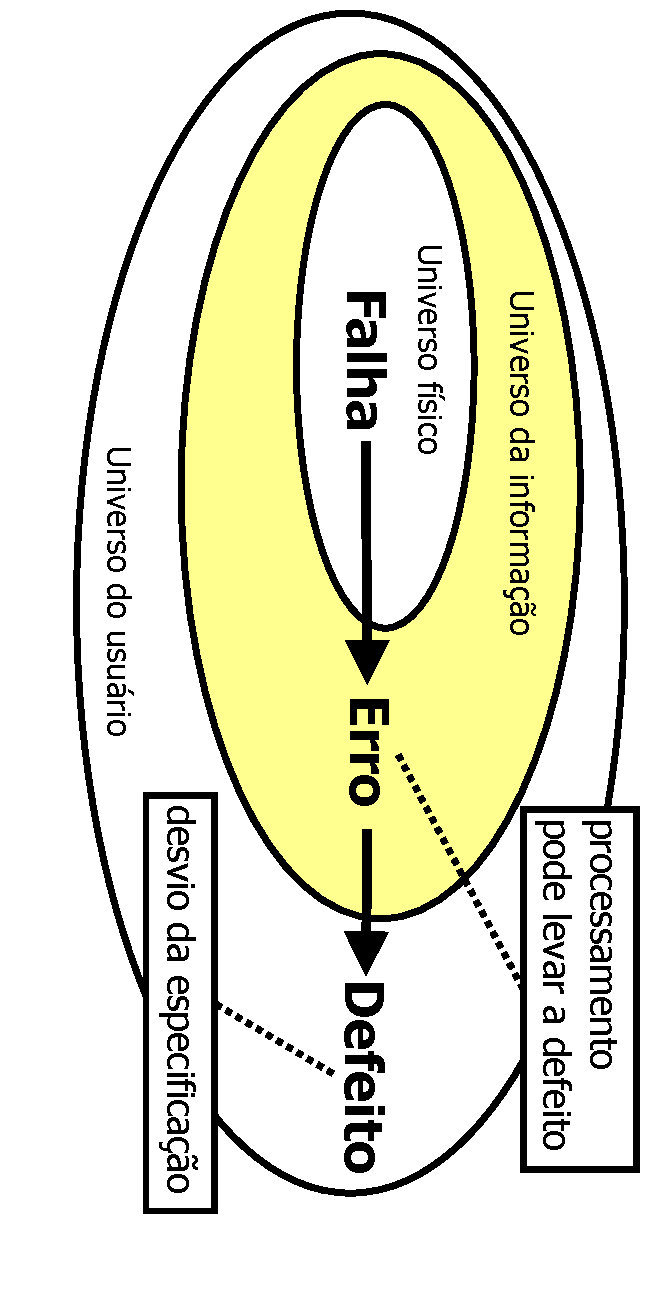
\includegraphics[height = 0.7 \linewidth, angle = 90]{figs/falha_erro_defeito.pdf}
\caption[Falha, erro e defeito]{Modelo de tr�s universos \cite{WEBER:2001}.}
\label{FIG:FED}
\end{figure}

Por exemplo, um chip de mem�ria que apresenta uma falha em um de seus bits (falha, universo f�sico) pode provocar uma interpreta��o errada da informa��o armazenada em uma estrutura de dados (erro, universo da informa��o) e como resultado o sistema pode negar autoriza��o de embarque para todos os passageiros de um v�o (defeito, universo do usu�rio).
� interessante observar que uma falha n�o leva, necessariamente, a um erro (aquela por��o da mem�ria pode nunca ser usada) e um erro n�o leva, necessariamente, a um defeito (no exemplo, a informa��o de v�o lotado poderia eventualmente ser obtida a partir de outros dados redundantes da estrutura).

Neste trabalho ser� utilizado apenas o conceito de falha, pois estamos interessados em diagnosticar um \emph{hardware}, parte do universo f�sico.

A descri��o de como alguma coisa pode falhar � o modelo de falha \cite{ADAMS:2003}. Esta descri��o pode ser feita em v�rios n�veis de abstra��o. No caso de circuitos integrados, existem os n�veis comportamental, funcional, l�gico, el�trico e geom�trico, mostrados na Figura \ref{FIG:ABSTRACTION}.

\begin{figure}[!ht]
\centering
\includegraphics[width = 0.7 \linewidth]{figs/abstraction_levels.png}
\caption[N�veis de abstra��o de falhas]{N�veis de abstra��o para modelagem de falhas.} \label{FIG:ABSTRACTION}
\end{figure}

O n�vel mais alto de abstra��o � o comportamental, que visa fazer uma descri��o em alto n�vel do sistema, geralmente auxiliada por uma \ac{HDL}.

Na modelagem em n�vel funcional, os circuitos s�o vistos como caixas pretas, isto �, apenas as entradas e sa�das s�o consideradas, n�o importando o trabalho interno realizado. Historicamente, esta � a modelagem mais utilizada para testes de mem�ria \cite{ADAMS:2003}.

No n�vel l�gico mais detalhes s�o acrescentados, passando a serem consideradas as portas l�gicas que comp�em os circuitos. Abaixo, est� o n�vel el�trico, onde as falhas s�o vistas nas opera��es dos transistores. Por fim, o modelo geom�trico se refere a todos os detalhes do processo de fabrica��o do circuito integrado, como tamanho e localiza��o das portas, dist�ncia entre c�lulas adjacentes, correntes de fuga entre po�os de dopagem, dentre outros \cite{ADAMS:2003}.

Os modelos de falhas funcionais s�o os mais empregados em testes e diagn�sticos de mem�ria \cite{ADAMS:2003}, porque n�o h� interesse na natureza das falhas, mas no seu efeito na funcionalidade dos circuitos. A partir deste ponto trataremos as falhas sempre a n�vel funcional.

%\subsection{Modelagem de Falhas em Mem�rias}

Os modelos de falhas cl�ssicos para circuitos digitais s�o \emph{Stuck-At Fault}, \emph{Bridging Fault}, \emph{Open Fault} e \emph{Delay Fault}. No entanto, eles n�o s�o suficientes para representar todas as falhas importantes em mem�rias, fazendo-se necess�rio definir erros mais espec�ficos para este tipo de circuito \cite{NAIR:1978, PAPACHRISTOU:1985}.

As falhas em mem�rias podem ser classificadas em tr�s categorias: falhas nas c�lulas de mem�ria, falhas no decodificador de endere�o e falhas din�micas. Cada umas destas categorias ser�o descritas nas pr�ximas se��es.

\subsection{Falhas na Matriz de C�lulas de Mem�ria}

As falhas nas c�lulas acontecem principalmente devido a curtos de metaliza��o e acoplamento capacitivo \cite{THATTE:1977}. Os principais tipos s�o \ac{SAF}, \ac{TF}, \ac{CF} e \ac{NPSF}, que s�o detalhados adiante.

Para descrever os estados das c�lulas de mem�ria com ou sem falhas, uma boa maneira � utilizar diagramas de Markov \cite{DAVID:1989}. Esses diagramas descrevem o comportamento de sistemas em um espa�o estado-tempo. Uma c�lula livre de qualquer defeito pode receber uma opera��o de escrita para qualquer estado e, quando lida, ret�m a informa��o na c�lula. A Figura \ref{FIG:MARKOV:FAUL_FREE} mostra o diagrama de Markov para uma c�lula de mem�ria livre de falhas. Adota-se neste trabalho a nota��o utilizada em \cite{ADAMS:2003}, onde as transi��es de estado representam as opera��es e $S_0$ e $S_1$ indicam que a c�lula est� no estado 0 ou 1, respectivamente. A transi��o R indica uma opera��o de leitura e W0 e W1 indicam opera��es de escrita para o estado 0 e 1, respectivamente.

\begin{figure}[!ht]
\centering
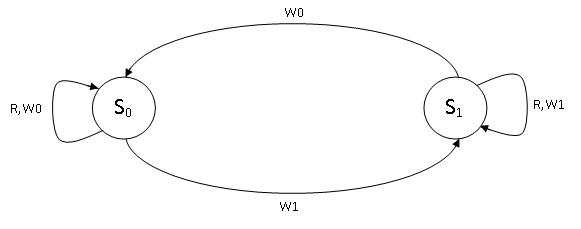
\includegraphics[width = 0.7 \linewidth]{figs/markov_fault_free.png}
\caption[Diagrama de c�lula sem falhas]{Diagrama de Markov para uma c�lula de mem�ria sem falhas. \cite{ADAMS:2003}} \label{FIG:MARKOV:FAUL_FREE}
\end{figure}

\subsubsection{\emph{Stuck-At Fault}}

Entre os modelos cl�ssicos de falhas em mem�rias, o mais conhecido e tamb�m o mais simples � o modelo \ac{SAF}, que � utilizado para indicar que uma c�lula est� presa em um determinado estado. A Figura ~\ref{FIG:MARKOV:SAFS} mostra o diagrama de Markov de uma falha do tipo \ac{SAF}. Independente do evento que ocorra, a c�lula se mant�m no seu estado atual.

\begin{figure}[!ht]
\centering
\subfigure[\label{FIG:MARKOV:STUCKAT_0}]{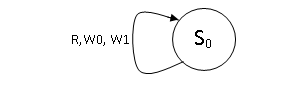
\includegraphics[width = 0.4 \linewidth]{figs/markov_stuckat_0.png}}
\subfigure[\label{FIG:MARKOV:STUCKAT_1}]{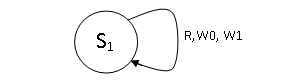
\includegraphics[width = 0.4 \linewidth]{figs/markov_stuckat_1.png}}
\caption[Diagramas \emph{Stuck-At}]{Diagramas de uma c�lula de mem�ria com \emph{Sutck-At} 0 (a) e \emph{Stuck-At} 1 (b). \cite{ADAMS:2003}} \label{FIG:MARKOV:SAFS}
\end{figure}

\subsubsection{Transition Fault}

Outro modelo simples de falha � o modelo \ac{TF}. De certa forma ele se parece com o \ac{SAF}, mas no caso de uma c�lula de mem�ria, ela ir� reter ambos os estados, mas uma vez escrita para um estado, ela n�o poder� fazer a transi��o de volta. Assim, quando a mem�ria � energizada a c�lula pode estar no estado ``0'' ou ``1'' e s� pode ser escrita em uma dire��o. A Figura ~\ref{FIG:MARKOV:TR} mostra o diagrama de Markov para uma falha do tipo \ac{TF}.

\begin{figure}[!ht]
\centering
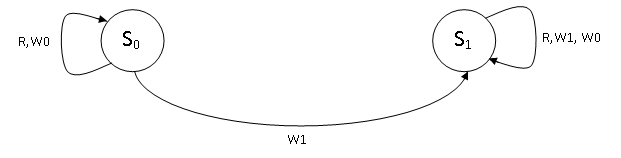
\includegraphics[width = 0.7 \linewidth]{figs/markov_transition.png}
\caption[Diagrama de \emph{Transition Fault}]{Diagrama de uma c�lula com \emph{Transition Fault}. \cite{ADAMS:2003}} \label{FIG:MARKOV:TR}
\end{figure}

\subsubsection{Coupling Fault}
\label{SEC:R3CF}

Para ilustrar uma \ac{CF} � necess�rio introduzir o diagrama de Markov para duas c�lulas. A Figura \ref{FIG:MARKOV:2FREE} mostra um par de c�lulas livres de falha, representadas pelos �ndices $i$ e $j$. Cada c�lula pode ser individualmente lida ou escrita para cada estado independentemente da outra, havendo um total de quatro estados poss�veis para o conjunto.

\begin{figure}[!ht]
\centering
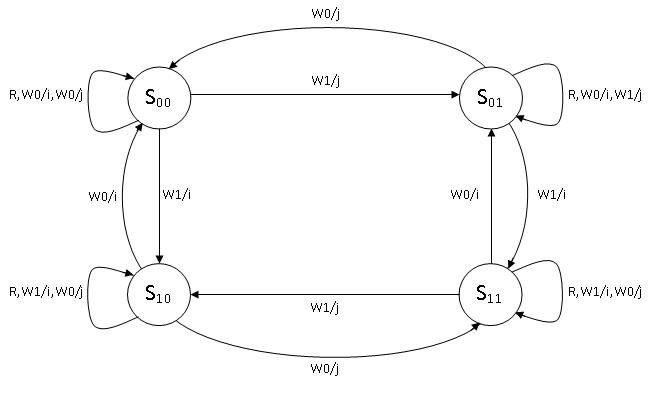
\includegraphics[width = 0.8 \linewidth]{figs/markov_2_cell.png}
\caption[Diagrama para duas c�lulas]{Diagrama para duas c�lulas sem falhas. \cite{ADAMS:2003}} \label{FIG:MARKOV:2FREE}
\end{figure}

Utiliza-se o modelo de falhas \ac{CF}, ou simplesmente acoplamento, quando h� um ou mais pares de c�lulas eletricamente acoplados, isto �, quando h� interfer�ncia eletromagn�tica entre elas. De forma simplificada, uma c�lula pode estar acoplada as c�lulas da sua vizinhan�a causando a transi��o para um estado err�neo ou uma falsa transi��o.

Os principais fatores que causam a falha \ac{CF} s�o a capacit�ncia m�tua e a corrente de fuga de uma c�lula para outra \cite{SUK:1981}. Papachristou \cite{PAPACHRISTOU:1985} a definiu formalmente como:
\begin{quote}
Quando uma opera��o de escrita que afeta a transi��o de 0 para 1 ou de 1 para 0 na c�lula $j$ muda o estado de outra c�lula $i$ ($i \neq j$), independente do conte�do da outra c�lula. Isto n�o implica que uma transi��o em $i$ mude o estado de $j$.
\end{quote}

Quando h� uma falha \ac{CF} entre as c�lulas, o diagrama de Markov do par passa a ser representado pela Figura \ref{FIG:MARKOV:CF}. Como descrito na defini��o, � poss�vel haver \ac{CF} em apenas um sentido, onde a c�lula provoca a falha na outra mas o oposto n�o acontece. No caso ilustrado, a falha s� ocorre quando a c�lula $i$ est� no estado 0 e a c�lula $j$ faz uma transi��o de 0 para 1. Caso a c�lula $i$, ao inv�s da $j$, fa�a uma transi��o de 0 para 1, nenhuma falha ser� provocada. A c�lula que causa a \ac{CF} � chamada de c�lula agressora \cite{ADAMS:2003} ou acopladora \cite{PAPACHRISTOU:1985} e a c�lula que sofre a falha � chamada de v�tima ou acoplada.
%??? precisa referenciar nos 2 momentos? ou s� no 2o? ou como est� mesmo?

\begin{figure}[!ht]
\centering
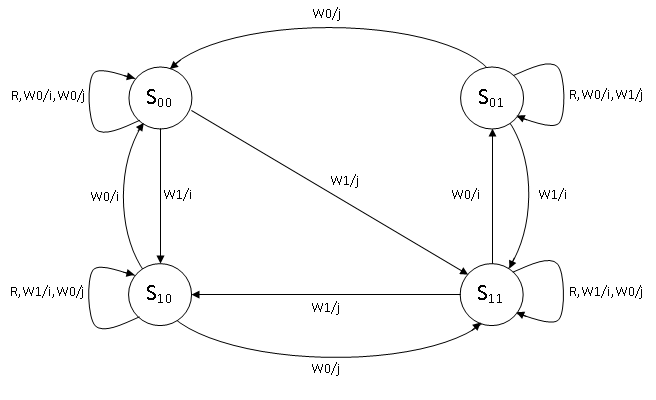
\includegraphics[width = 0.8 \linewidth]{figs/markov_coupling.png}
\caption[Diagrama de \emph{Coupling fault}]{Diagrama para duas c�lulas com \ac{CF}. \cite{ADAMS:2003}} \label{FIG:MARKOV:CF}
\end{figure}

A falha \ac{CF} pode se apresentar nos seguinte tipos \cite{RAGHURAMAN:2005}:

\begin{enumerate}
  \item \textbf{Inversion Coupling Fault}: Uma transi��o na c�lula agressora inverte o conte�do da c�lula v�tima;
  \item \textbf{Idempotent Coupling Fault}: Uma transi��o na c�lula agressora for�a um valor l�gico fixo na c�lula v�tima;
  \item \textbf{State Coupling Fault}: A c�lula v�tima � for�ada para certo estado apenas se a c�lula agressora estiver em  determinado estado. Tamb�m conhecida como \ac{PSF}.
\end{enumerate}

Um conjunto de $k$ c�lulas � dito estar $k$-acoplado (\emph{$k$-coupled}) se uma transi��o em uma c�lula causa uma transi��o em outra c�lula do conjunto quando as outras $k-2$ c�lulas est�o em certo estado. Um caso especial chamado de \emph{restricted $k$-coupling} � convenientemente definido como um \emph{$k$-coupling} onde as $k-1$ c�lulas n�o possuem acoplamento entre si. Devido a enorme complexidade dos modelos de falhas para $k$ maior que 3, apenas falhas \emph{2-coupling} e \emph{restricted 3-coupling} t�m sido investigadas na literatura \cite{PAPACHRISTOU:1985} \cite{ADAMS:2003}.

\subsubsection{Neighborhood Pattern Sensitive Fault}

O modelo \ac{NPSF}, se apresenta sobre uma c�lula chamada de c�lula-base e sua vizinhan�a f�sica. Na realidade, o \ac{NPSF} � um caso especial de \emph{$k$-coupling} em que as $k-1$ c�lulas agressoras est�o restritas a uma vizinhan�a fixa em proximidade f�sica da c�lula base. Este modelo � bastante estudado por ser mais comum que acoplamentos entre c�lulas distantes \cite{PETRU:2002}.

\subsection{Falhas no Decodificador de Endere�o}

O decodificador � um circuito de l�gica combinacional simples que seleciona uma �nica c�lula de mem�ria para um dado endere�o. Qualquer falha ocorrida no decodificador far� com que ele se comporte de umas das maneiras:

\begin{enumerate}
  \item O decodificador n�o ir� acessar a c�lula endere�ada. Al�m disto, ele pode acessar c�lulas n�o endere�adas;
  \item O decodificador ir� acessar m�ltiplas c�lulas, incluindo a c�lula endere�ada.
\end{enumerate}

No caso de m�ltiplos acessos (ii), podemos ver a falha como uma falha na matriz de c�lulas, isto �, como uma \ac{CF} entre as c�lulas afetadas. No caso (i), a c�lula que deveria ter sido selecionada pode ser vista como \emph{stuck at} 0 ou \emph{stuck at} 1, dependendo da l�gica utilizada.

Em todos os casos, podemos visualizar as falhas no decodificador como falhas na matriz de c�lulas da mem�ria \cite{NAIR:1978} \cite{PETRU:2002}.

\subsection{Falhas Din�micas}

As falhas din�micas em mem�rias s�o tamb�m chamadas de falhas na l�gica de escrita e leitura (\emph{Read/Write Logic Fault}). Algumas linhas dos circuitos de escrita e leitura podem estar em \emph{stuck at} 0 ou \emph{stuck at} 1. Neste caso, podemos considerar a falha como uma \ac{SAF} nas c�lulas afetadas por essas linhas. As linhas de entrada ou sa�da de dados das c�lulas podem conter curtos ou acoplamentos capacitivos entre elas. Estas falhas podem ser visualizadas como \ac{CF} entre as c�lulas correspondentes.

Portanto, para testes de \ac{RAM}, todas os tipos de falhas podem ser representados apenas pelos modelos de falhas na matriz de c�lulas de mem�ria, isto � \ac{SAF}, \ac{TF}, \ac{CF} e \ac{NPSF} \cite{NAIR:1978,PETRU:2002}. 
    %%% Se��o 2.2 Tipos de testes de mem�ria:
    \section{Tipos de testes de mem�ria}
\label{SEC:TESTES}

Uma mem�ria guarda zeros e uns. Se zeros s�o escritos em todos os endere�os da mem�ria e lidos de todos os endere�os, ent�o metade das falhas foram cobertas, certo? Na realidade, n�o.

O teste mencionado � um dos testes mais simples existentes. � chamado de padr�o zero-um (\emph{zero-one pattern}) ou padr�o trivial. %Apesar da simplicidade, este teste tem cobertura de 100\% das falhas \ac{SAF}, por�m � incapaz de detectar a maior parte dos outros modelos \cite{ADAMS:2003}.
Apesar da simplicidade e deste teste ter cobertura de 100\% das falhas \ac{SAF}, ele � incapaz de detectar a maior parte dos outros tipos de falhas \cite{ADAMS:2003}. A situa��o descrita na Figura \ref{FIG:ARRAY_NO_01} � um exemplo onde este teste n�o � suficiente. Neste caso h� uma falha nos decodificadores de forma que, independente do endere�o selecionado, sempre a mesma c�lula � acessada, tanto na escrita quanto na leitura.

\begin{figure}[!htb]
\centering
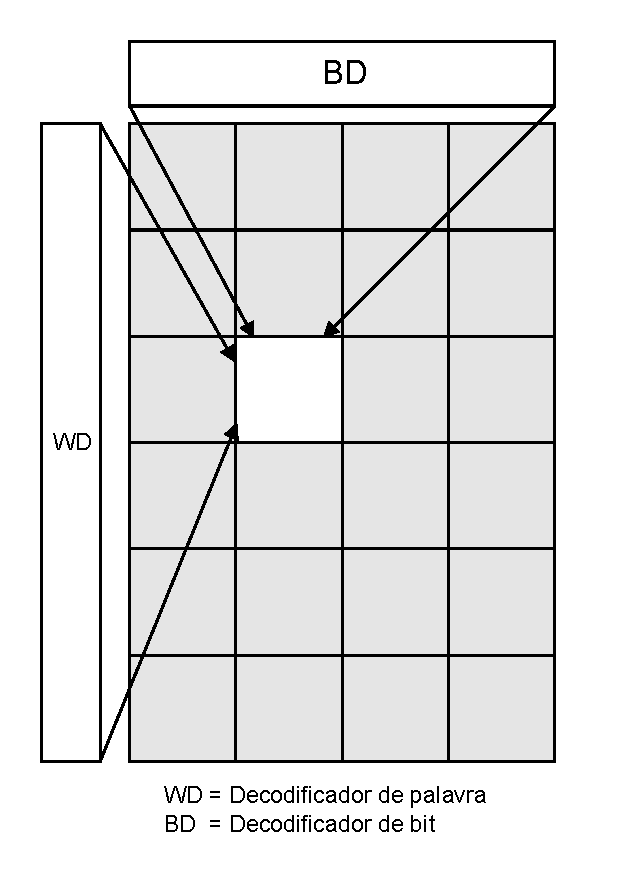
\includegraphics[width = 0.6 \linewidth]{figs/array_no_01.pdf}
\caption[Erro n�o detect�vel por padr�o zero-um]{Erro n�o detect�vel por padr�o zero-um.} \label{FIG:ARRAY_NO_01}
\end{figure}

Para que seja poss�vel testar mem�rias de forma mais completa, � necess�rio usar uma combina��o de padr�es de teste (\emph{patterns}), onde cada padr�o tem a capacidade de detectar certos tipos de falhas. Nenhum padr�o sozinho � suficiente para testar uma mem�ria por completo \cite{DEAN:1994}. Padr�es s�o a ess�ncia dos testes de mem�ria \cite{ADAMS:2003}.

Para a descri��o de testes, adota-se uma nota��o baseada em \cite{ADAMS:2003}. A Tabela \ref{TAB:01} mostra a representa��o do teste zero-um citado anteriormente. Cada linha indica uma sequ�ncia de opera��es que deve ser aplicada a cada c�lula antes de prosseguir para a pr�xima sequ�ncia. A estas sequ�ncias, tamb�m d�-se o nome de elementos de teste \cite{PAPACHRISTOU:1985}. No exemplo temos quatro elementos, do 1 ao 4, cada um com apenas uma opera��o. As opera��es podem ser:

\begin{itemize}
  \item W0 escrever 0 na c�lula
  \item R0 ler estado da c�lula, esperado 0
  \item W1 escrever 1 na c�lula
  \item R1 ler estado da c�lula, esperado 1
\end{itemize}

Ao final das opera��es em um endere�o, a passagem de uma c�lula para outra pode ser de forma ascendente, representada pelo s�mbolo $\Uparrow$, descendente, representada por $\Downarrow$ ou em qualquer dire��o, representada por $\Updownarrow$.

\begin{table}[!ht]
\caption{\emph{Zero-Ones Pattern.}}
\centering
\label{TAB:01}
\begin{tabular}{| c | l r |}
\hline
1 & W0 & $\Updownarrow$ \\
2 & R0 & $\Updownarrow$ \\
3 & W1 & $\Updownarrow$ \\
4 & R1 & $\Updownarrow$ \\
\hline
\end{tabular}
\end{table}

%A Complexidade de um algoritmo consiste na quantidade de trabalho necess�ria para a sua execu��o, expressa em fun��o das opera��es fundamentais, as quais variam de acordo com o algoritmo, e em fun��o do volume de dados. � medida segundo um modelo matem�tico que sup�e que este vai trabalhar sobre uma entrada (massa de dados) de tamanho N. O processo de execu��o de um algoritmo pode ser dividido em etapas elementares denominadas passos (n�mero fixo de opera��es b�sicas, tempo constante, opera��o de maior freq��ncia chamada dominante). O n�mero de passos de um algoritmo � considerado como o n�mero de execu��es da opera��o dominante em fun��o das sa�das, desprezando-se constantes aditivas ou multiplicativas.

Atrav�s desta drescri��o tamb�m � possivel medir a complexidade do teste. Isto �, quantos ciclos s�o necess�rios para executar todo o teste. Supondo que uma opera��o de escrita ou leitura possa ser realizada em um ciclo, o teste apresentado possui uma complexidade 4$N$, onde $N$ � a quantidade de c�lulas ou o tamanho da mem�ria. Este teste � dito ser de ordem $N$, representado por $O(N)$. Um teste de complexidade 14$N\log_2(N)$ possui ordem $O(N\log_2(N))$. O conceito de complexidade � importante pois os chips de mem�ria crescem constantemente seguindo a Lei de Moore. Isto faz com que testes mais complexos levem tempos impratic�veis para os tamanhos e velocidades das mem�rias atuais.

Tomando como exemplo uma mem�ria com tempo de acesso de 1,25 ns\footnote{Tempo de acesso retirado do \emph{datasheet} de uma mem�ria DDR3 SDRAM SODIMM. \cite{MICRON:2008}.}, a Tabela \ref{TAB:TEMPOS} mostra os tempos de execu��o de supostos testes de diferentes complexidades em diferentes tamanhos de mem�ria.

\begin{table}[!ht]
\caption{Tempos de execu��o em mem�ria com tempo de acesso de 1,25 ns.}
\centering
\label{TAB:TEMPOS}
\begin{tabular}{|l|l|l|l|l|}
\hline
Tamanho & \multicolumn{4}{c|}{Complexidade} \\
\cline{2-5}
$N$ & $N$ & $N\log_2(N)$ & $N^{3/2}$ & $N^2$ \\
\hline
1 KB & 1,28 $\mu$s & 12,8 $\mu$s & 40,96 $\mu$s & 1,31 ms \\
4 KB & 5,12 $\mu$s &  61,44 $\mu$s & 327,68 $\mu$s & 20,97 ms \\
16 KB & 20,48 $\mu$s & 286,72 $\mu$s & 2,62 ms & 335,54 ms \\
64 KB & 81,92 $\mu$s & 1,31 ms & 20,97 ms & 5,37 s \\
256 KB & 327,68 $\mu$s & 5,90 ms & 167,77 ms &  1,43 min \\
1 MB & 1,31 ms & 26,21 ms & 1,34 s &  22,91 min \\
4 MB & 5,24 ms & 115,34 ms & 10,74 s &  6,11 h \\
16 MB & 20,97 ms & 503,32 ms &  1,43 min &  4,07 dias \\
64 MB & 83,89 ms & 2,18 s &  11,45 min &  65,16 dias \\
256 MB & 335,54 ms & 9,40 s &  1,53 h &  2,86 anos \\
1 GB & 1,34 s & 40,27 s &  12,22 h &  45,70 anos \\
2 GB & 2,68 s & 1,39 min &  1,44 dia &  182,79 anos \\
4 GB & 5,37 s & 2,86 min &  4,07 dias &  731,18 anos \\
\hline
\end{tabular}
\end{table}

� importante notar que em testes reais os tempos s�o m�ltiplos desses valores. Um teste de complixadade 8$N$, por exemplo, iria levar $8 \cdot 1,34 s = 10,72 s$ para testar 1 GB de mem�ria, pois, pela tabela, leva-se $1,34 s$ para executar cada $N$ opera��es. Assim, apenas testes de complexidade at� $O(N\log_2(N))$ s�o aceit�veis \cite{RAGHURAMAN:2005}.

Os padr�es de testes de mem�ria s�o comumente categorizados como caminhantes (\emph{walking}), marchantes (\emph{marching}) e galopantes (\emph{galloping}) \cite{VANDEGOOR:1998}.

\subsubsection{Testes Caminhantes (\emph{Walking})}

Um teste � dito ser caminhante (\emph{walking}) quando, em cada momento, h� apenas uma c�lula em um estado diferente de todas as outras.

Inicialmente a mem�ria � totalmente preenchida com um padr�o, ent�o as opera��es de escrita e leitura s�o realizadas em uma c�lula e ao final da sequ�ncia, a c�lula deve voltar ao estado inicial. A tabela \ref{TAB:WALKING} mostra um exemplo de elemento para um teste caminhante.

\begin{table}[!ht]
\caption{Exemplo de \emph{walking}.}
\centering
\label{TAB:WALKING}
\begin{tabular}{| c | l r |}
\hline
1 & R0, W1, R1, W0 & $\Uparrow$ \\
\hline
\end{tabular}
\end{table}

O que caracteriza este elemento como caminhante � que a �ltima opera��o de escrita (W0) retorna a c�lula para o estado em que ela se encontrava antes do in�cio da sequ�ncia (que pode ser notado pela leitura R0).

\subsubsection{Testes Marchantes (\emph{Marching})}

Um padr�o em marcha (\emph{marching pattern}) � quando o teste muda o estado da c�lula testada e n�o a retorna para o estado anterior. Assim, antes de come�ar o teste, a mem�ria est� preenchida com um certo padr�o, ap�s uma sequ�ncia percorrer metade da mem�ria, metade estar� com o padr�o inicial e a outra metade estar� com o padr�o escrito pelo teste. Um exemplo de um elemento \emph{march} � mostrado na tabela \ref{TAB:MARCHING}.

\begin{table}[!ht]
\caption{Exemplo de \emph{marching}.}
\centering
\label{TAB:MARCHING}
\begin{tabular}{| c | l r |}
\hline
1 & R0, W1, R1 & $\Downarrow$ \\
\hline
\end{tabular}
\end{table}

O que diferencia este elemento de um caminhante � que sua �ltima escrita n�o � necessariamente para o valor inicial da c�lula.

\subsubsection{Testes Galopantes (\emph{Galloping})}

Enquanto os padr�es caminhantes e marchantes s�o orientados a dado, o galopante (\emph{galloping pattern}) � orientado a endere�o. A diferen�a � que esta categoria faz uma checagem do tipo \emph{ping-pong} entre a c�lula base (c�lula atualmente testada) e todas as outras da matriz. Como em cada opera��o � preciso percorrer toda a mem�ria, este tipo de teste leva muito tempo para ser realizado. Sua complexidade � da ordem de $O(N^2)$, o que � bastante, comparada a complexidade de ordem $N$ dos outros dois tipos apresentados.

A cobertura de falhas dos testes galopantes � consideravelmente maior, no entanto o excesso de tempo faz com que sua utiliza��o seja invi�vel. Como mostrado na Tabela \ref{TAB:TEMPOS}, um teste que levaria alguns minutos com padr�es caminhantes ou marchantes, poderia precisar de anos para ser conclu�do com um padr�o galopante.

\subsection{Testes Conhecidos}

Desde metade do s�culo XX muitos padr�es para testes de mem�ria t�m sido propostos. Ao longo do tempo eles foram aperfei�oados tanto no sentido de aprimorar a cobertura de falhas quanto no sentido de reduzir a quantidade de opera��es realizadas. Neste cap�tulo trataremos apenas dos algoritmos mais utilizados pela ind�stria e referenciados na literatura.

\subsubsection{S�rie March}

Existe um conjunto tradicional de testes do tipo marchante identificados por letras. Destes, o March C- ganhou destaque em muitos trabalhos por ser muito simples e ainda assim poderoso na detec��o de falhas. Seu nome � dado por ser uma otimiza��o de outro padr�o, chamado March C, onde algumas inefici�ncias foram eliminadas. Como pode ser visto na Tabela \ref{TAB:MARCHC-}, o March C- � um teste $10N$. Ele � capaz de detectar todas as falhas do tipo \ac{SAF}, \emph{idempotent} \ac{CF}, \ac{TF} e parte das falhas de alguns outro tipos \cite{ADAMS:2003}. De acordo com \cite{PETRU:2002}, 81,25\% das falhas \ac{CF} simples entre 2 c�lulas s�o detectadas por este teste.

\begin{table}[!ht]
\caption{\emph{March C- pattern.}}
\centering
\label{TAB:MARCHC-}
\begin{tabular}{| c | l r |}
\hline
1 & W0 & $\Updownarrow$ \\
2 & R0, W1 & $\Uparrow$ \\
3 & R1, W0 & $\Uparrow$ \\
4 & R0, W1 & $\Downarrow$ \\
5 & R1, W0 & $\Downarrow$ \\
6 & R0 & $\Updownarrow$ \\
\hline
\end{tabular}
\end{table}

Uma melhoria do March C- foi proposta por \cite{ADAMS:2003}. Chamado de Enhanced March C-, o teste, descrito na tabela \ref{TAB:EMARCHC-}, executa $18N$ opera��es e detecta algumas falhas al�m das j� cobertas pelo March C-.

\begin{table}[!ht]
\caption{\emph{Enhanced March C- pattern.}}
\centering
\label{TAB:EMARCHC-}
\begin{tabular}{| c | l r |}
\hline
1 & W0 & $\Updownarrow$ \\
2 & R0, W1, R1, W1 & $\Uparrow$ \\
3 & R1, W0, R0, W0 & $\Uparrow$ \\
4 & R0, W1, R1, W1 & $\Downarrow$ \\
5 & R1, W0, R0, W0 & $\Downarrow$ \\
6 & R0 & $\Updownarrow$ \\
\hline
\end{tabular}
\end{table}

\subsubsection{Moving Invertion}

Outro padr�o muito conhecido � o \ac{MOVI}. Seu funcionamento � um pouco mais complexo que os testes do tipo marchante.

Inialmente toda a mem�ria � preenchida com zeros. Ent�o repete-se o seguinte procedimeno: uma palavra � lida; um bit � escrito para 1; a palavra � lida novamente. Isto se repete at� que todos os bits da palavra estejam com o valor 1 e � feito para todas as palavras da mem�ria. Ap�s completar toda a mem�ria, a opera��o inversa � aplicada: uma palavra � lida; um bit � escrito para 0; a palavra � lida novamente. At� que todas as palavras estejam com o valor 0 novamente.

Todo este procedimento � repetido $n$ vezes, onde $n$ � o tamanho do barramento de endere�o. No entanto, o \ac{MOVI} utiliza uma forma de endere�amento diferente dos padr�es vistos at� aqui, chamada de endere�amento n�o linear. Para cada repeti��o o endere�o � deslocado de forma circular para a esquerda e considera-se o bit $n$ como o \ac{LSB}. Por exemplo, na segunda repeti��o o \ac{LSB} ser� o bit $1$ e o endere�amento segue a ordem mostrada na tabela \ref{TAB:ENDMOVI}.

\begin{table}[!ht]
\caption{\emph{Endere�amento do MOVI na segunda itera��o (LSB = bit 1).}}
\centering
\label{TAB:ENDMOVI}
\begin{tabular}{| c |}
\hline
000\ldots0\underline{0}0 \\
000\ldots0\underline{1}0 \\
000\ldots1\underline{0}0 \\
000\ldots1\underline{1}0 \\
\vdots \\
111\ldots1\underline{1}0 \\
000\ldots0\underline{0}1 \\
000\ldots0\underline{1}1 \\
\vdots \\
\hline
\end{tabular}
\end{table}

Este teste realiza $12nN\log_2(N)$ opera��es e detecta falhas de endere�amento, \ac{SAF}, \ac{TF} e problemas com o tempo de acesso \cite{PHAN:2002}.

\subsubsection{Nair}

Um dos grandes trabalhos em testes de mem�ria � \cite{NAIR:1978}, onde foram propostos dois algoritmos com boa efici�ncia e cobertura de falhas. O primeiro, chamado de algoritmo A, � de ordem $O(N)$ e detecta todas a falhas simples e acoplamentos at� 2 c�lulas. O segundo, algortimo B, � de ordem $O(N\log_2(N))$, mas detecta as mesmas falhas do algortimo A com o acr�scimo de acoplamentos entre 3 c�lulas do tipo restrito (\emph{restricted 3-coupling faults}, ver final da sess�o \ref{SEC:R3CF}).

\subsubsection{Papachristou}

O Papachristou � um dos testes mais conhecidos e utilizados e tamb�m um dos que apresenta melhor cobertura de falhas com complexidade pratic�vel. Proposto por \cite{PAPACHRISTOU:1985}, inspirado nos algoritmos A e B de \cite{NAIR:1978}, o autor desenvolveu um algortimo capaz de detectar todas as falhas detect�veis por A e B, al�m algumas do tipo \ac{NPSF}. O teste pode ser dividido em duas etapas, uma de ordem $O(N)$ com a mesma cobertura que o algoritmo A e a segunda de ordem $N\log_2(N)$. No total, s�o necess�rias $38 N + 24 N \log(N)$ opera��es.

O teste de $38N$ opera��es � do tipo marchante e ser� chamado de Papachristou 1 ou parcial neste trabalho. Ele � equivalente ao Nair A quanto �s falhas detectadas e seus elementos s�o descritos na tabela \ref{TAB:PAPACHRISTOU1}.

\begin{table}[!ht]
\caption{Algoritmo Papachristou 1.}
\centering
\label{TAB:PAPACHRISTOU1}
\begin{tabular}{| c | l r |}
\hline
1 & W0 & $\Updownarrow$ \\
2 & R0, W1, R1 & $\Uparrow$ \\
3 & R1, W0, R0 & $\Uparrow$ \\
4 & R0, W1, W0 & $\Uparrow$ \\
5 & R0, W1 & $\Uparrow$ \\
6 & R1, W0, W1 & $\Uparrow$ \\
7 & R1, W0 & $\Uparrow$ \\
8 & R0, W1, W0 & $\Uparrow$ \\
9 & R0, W1 & $\Downarrow$ \\
10 & R1, W0 & $\Downarrow$ \\
11 & R0, W1, W0 & $\Downarrow$ \\
12 & R0, W1 & $\Downarrow$ \\
13 & R1, W0, W1 & $\Downarrow$ \\
14 & R1, W0 & $\Downarrow$ \\
15 & R0, W1, W0 & $\Downarrow$ \\
16 & R0 & $\Updownarrow$ \\
\hline
\end{tabular}
\end{table}

O Papachristou 2 ou completo, como ser� chamado o procedimento inteiro, consiste na aplica��o do teste anterior seguido de um segundo teste com as opera��es descritas na tabela \ref{TAB:PAPACHRISTOU2} utilizando o mesmo endere�amento n�o linear do \ac{MOVI}. Um ponto importante � que este teste divide a mem�ria em duas metades e as opera��es s�o realizadas na metade superior ou na inferior, definidas pelo \ac{MSB} do endere�o ap�s o deslocamento c�clico do endere�amento n�o linear.

\begin{table}[!ht]
\caption{Segunda etapa do algoritmo Papachristou 2.}
\centering
\label{TAB:PAPACHRISTOU2}
\begin{tabular}{| c | l r |}
\hline
1 & R0, W1 & $\Uparrow t$ \\
2 & R0 & $\Uparrow b$ \\
3 & R0, W1 & $\Uparrow b$ \\
4 & R1 & $\Uparrow t$ \\
5 & R1, W0 & $\Uparrow t$ \\
6 & R1 & $\Uparrow b$ \\
7 & R1, W0 & $\Uparrow b$ \\
8 & R0 & $\Uparrow t$ \\
9 & R0, W1 & $\Downarrow b$ \\
10 & R0 & $\Downarrow t$ \\
12 & R0, W1 & $\Downarrow t$ \\
12 & R1 & $\Downarrow b$ \\
13 & R1, W0 & $\Downarrow b$ \\
14 & R1 & $\Downarrow t$ \\
15 & R1, W0 & $\Downarrow t$ \\
16 & R0 & $\Downarrow b$ \\
\hline
\end{tabular}
\end{table}

\subsubsection{MT}

Nas �ltimas d�cadas pouco se tem avan�ado em rela��o � cobertura de falhas dos algoritmos de teste de mem�ria. As novas propostas concentram-se na cria��o de padr�es muito espec�ficos para tipos particulares de falhas, al�m do desenvolvimento de \emph{hardware} e \emph{cores} acoplados ao pr�prio circuito de mem�ria para facilitar a aplica��o de testes autom�ticos. Estes \emph{hardwares} fazem parte de um conceito chamado de \ac{DFT}, que � um conjunto de t�cnicas que adicionam certas caracter�sticas de testabilidade a circuitos microeletr�nicos. Em mem�rias, � utilizado particularmente circuitos de \ac{BIST}, que s�o mecanismos que permitem ao hardware fazer testes de forma autom�tica.

Entre os padr�es mais recentes ganha destaque um algoritmo chamado de MT \cite{PETRU:2002}. � um teste do tipo marchante com apenas $36N$ opera��es, mas que detecta todas as falhas detectadas por Papachristou 2, de ordem $O(N\log_2(N))$, al�m de cobrir todas as falhas do tipo \emph{3-coupling fault} entre c�lulas adjacentes, n�o apenas as do tipo restrito. Em outras palavras, este teste � capaz de detectar todas as falhas \ac{NPSF} entre 3 c�lulas.

Para isto, a descri��o do teste segue uma abordagem um pouco diferente. Ao inv�s de escrever sempre o mesmo valor em toda a mem�ria, as c�lulas s�o preenchidas com os padr�es de fundos mostrados nas tabelas \ref{TAB:MTBACKGROUNDS}, nomeados de $I_1$ a $I_6$.

\begin{table}[!ht]
\centering
\subtable[\label{TAB:I1}]{
\begin{tabular}{| c | c | c | c |}
\multicolumn{4}{c}{$I_1$} \\
\hline
0 & 0 & 0 & 0 \\
\hline
0 & 0 & 0 & 0 \\
\hline
0 & 0 & 0 & 0 \\
\hline
0 & 0 & 0 & 0 \\
\hline
\end{tabular}
}
\subtable[\label{TAB:I2}]{
\begin{tabular}{| c | c | c | c |}
\multicolumn{4}{c}{$I_2$} \\
\hline
0 & 1 & 0 & 1 \\
\hline
0 & 1 & 0 & 1 \\
\hline
0 & 1 & 0 & 1 \\
\hline
0 & 1 & 0 & 1 \\
\hline
\end{tabular}
}
\subtable[\label{TAB:I3}]{
\begin{tabular}{| c | c | c | c |}
\multicolumn{4}{c}{$I_3$} \\
\hline
1 & 1 & 1 & 1 \\
\hline
1 & 1 & 1 & 1 \\
\hline
1 & 1 & 1 & 1 \\
\hline
1 & 1 & 1 & 1 \\
\hline
\end{tabular}
}
\subtable[\label{TAB:I4}]{
\begin{tabular}{| c | c | c | c |}
\multicolumn{4}{c}{$I_4$} \\
\hline
1 & 0 & 1 & 0 \\
\hline
1 & 0 & 1 & 0 \\
\hline
1 & 0 & 1 & 0 \\
\hline
1 & 0 & 1 & 0 \\
\hline
\end{tabular}
}
\subtable[\label{TAB:I5}]{
\begin{tabular}{| c | c | c | c |}
\multicolumn{4}{c}{$I_5$} \\
\hline
0 & 0 & 0 & 0 \\
\hline
1 & 1 & 1 & 1 \\
\hline
0 & 0 & 0 & 0 \\
\hline
1 & 1 & 1 & 1 \\
\hline
\end{tabular}
}
\subtable[\label{TAB:I6}]{
\begin{tabular}{| c | c | c | c |}
\multicolumn{4}{c}{$I_6$} \\
\hline
1 & 1 & 1 & 1 \\
\hline
0 & 0 & 0 & 0 \\
\hline
1 & 1 & 1 & 1 \\
\hline
0 & 0 & 0 & 0 \\
\hline
\end{tabular}
}
\caption{Padr�es de fundo no algoritmo MT.} \label{TAB:MTBACKGROUNDS}
\end{table}

O teste consistem em preencher a mem�ria com estes padr�es e executar uma sequ�ncia de opera��es de leitura e escrita. Diferente dos outros testes apresentados, os elementos utilizados para sua descri��o usam as opera��es $I_x$, R e WC (tabela \ref{TAB:MT}), que significam respectivamente escrever o padr�o de fundo $I_x$ em toda a mem�ria, ler 0 ou 1 dependendo do padr�o e do endedre�o atual e escrever o complemento do valor presente na c�lula.

\begin{table}[!ht]
\caption{\emph{MT pattern.}}
\centering
\label{TAB:MT}
\begin{tabular}{| c | l r |}
\hline
1 & $I_1$ & $\Updownarrow$ \\
2 & R, WC, R, WC & $\Uparrow$ \\
3 & R & $\Updownarrow$ \\
4 & $I_2$ & $\Updownarrow$ \\
5 & R, WC, R, WC & $\Uparrow$ \\
6 & R & $\Updownarrow$ \\
7 & $I_3$ & $\Updownarrow$ \\
8 & R, WC, R, WC & $\Uparrow$ \\
9 & R & $\Updownarrow$ \\
10 & $I_4$ & $\Updownarrow$ \\
11 & R, WC, R, WC & $\Uparrow$ \\
12 & R & $\Updownarrow$ \\
13 & $I_5$ & $\Updownarrow$ \\
14 & R, WC, R, WC & $\Uparrow$ \\
15 & R & $\Updownarrow$ \\
16 & $I_6$ & $\Updownarrow$ \\
17 & R, WC, R, WC & $\Uparrow$ \\
18 & R & $\Updownarrow$ \\
\hline
\end{tabular}
\end{table}

\subsubsection{GALPAT}

O teste tomado como refer�ncia, em termos de cobertura de falhas, � um algoritmo do tipo galopante chamando GALPAT \cite{NAIR:1978} \cite{PAPACHRISTOU:1985} \cite{RIEDEL:1995}. Ele cobre praticamente todos os tipos de falhas conhecidos, no entanto � considerado um teste meramente te�rico, pois sua complexidade � de ordem $O(N^2)$.

Para a implementa��o de testes de mem�ria, n�o basta conhecer os algortimos. Estes descrevem apenas o conjunto de opera��es capazes de detectar as falhas, por�m uma s�rie caracter�sticas do \ac{SO} precisa ser levada em considere��o. As caracter�sticas pertinentes ao Linux ser�o apresentadas na pr�xima se��o. 
    %%% Se��o 2.3 Gerenciamento de mem�ria do Linux:
    \section{Gerenciamento de mem�ria do Linux}
\label{SEC:LINUXMM}

Para projetar um bom teste que execute sobre toda a abstra��o imposta por um \ac{SO}, � necess�rio conhecer a fundo como o \emph{hardware} em quest�o � tratado pelo sistema. No caso da mem�ria, o respons�vel por esta manipula��o � o subsistema chamado de gerenciador de mem�ria. Ele � o mecanismo que prover meios para, dinamicamente, alocar por��es de mem�ria para os programas que solicitarem e liber�-la para reuso quando n�o forem mais necess�rias \cite{KNUTH:1997}. No Linux, o subsistema respons�vel pelo gerenciamento de mem�ria � o \ac{LinuxMM} \cite{LINUXMM:2009}.

\subsection{Mem�ria Virtual}

Os gerenciadores de mem�ria utilizam o conceito de mem�ria virtual para melhorar a eficiencia em sistemas multitarefas. A mem�ria virtual permite que o gerenciador organize a mem�ria independentemente da disposi��o f�sica dos circuitos. As aplica��es acessam a mem�ria apenas atrav�s de endere�os virtuais. Cada vez que � feita uma tentativa de acesso, o gerenciador traduz o endere�o virtual em um endere�o f�sico, que corresponde a localiza��o do dado como armazenado no hardware \cite{GLASER:1965}.

Os \emph{chips} de mem�ria s�o fabricados como uma matriz de c�lulas e s�o montados, tipicamente, divididos em bancos, que nada mais s�o que placas contendo alguns \ac{CI}s de mem�ria e controladores, como na Figura \ref{FIG:MEM_TOPOLOGIA}. Gra�as a mem�ria virtual, a aplica��o acessa sua por��o de mem�ria como um simples vetor de bytes unidimensional, como mostrado na Figura \ref{FIG:MEM_VECTOR}.

\begin{figure}[!ht]
\centering
\subfigure[\label{FIG:MEM_TOPOLOGIA}]{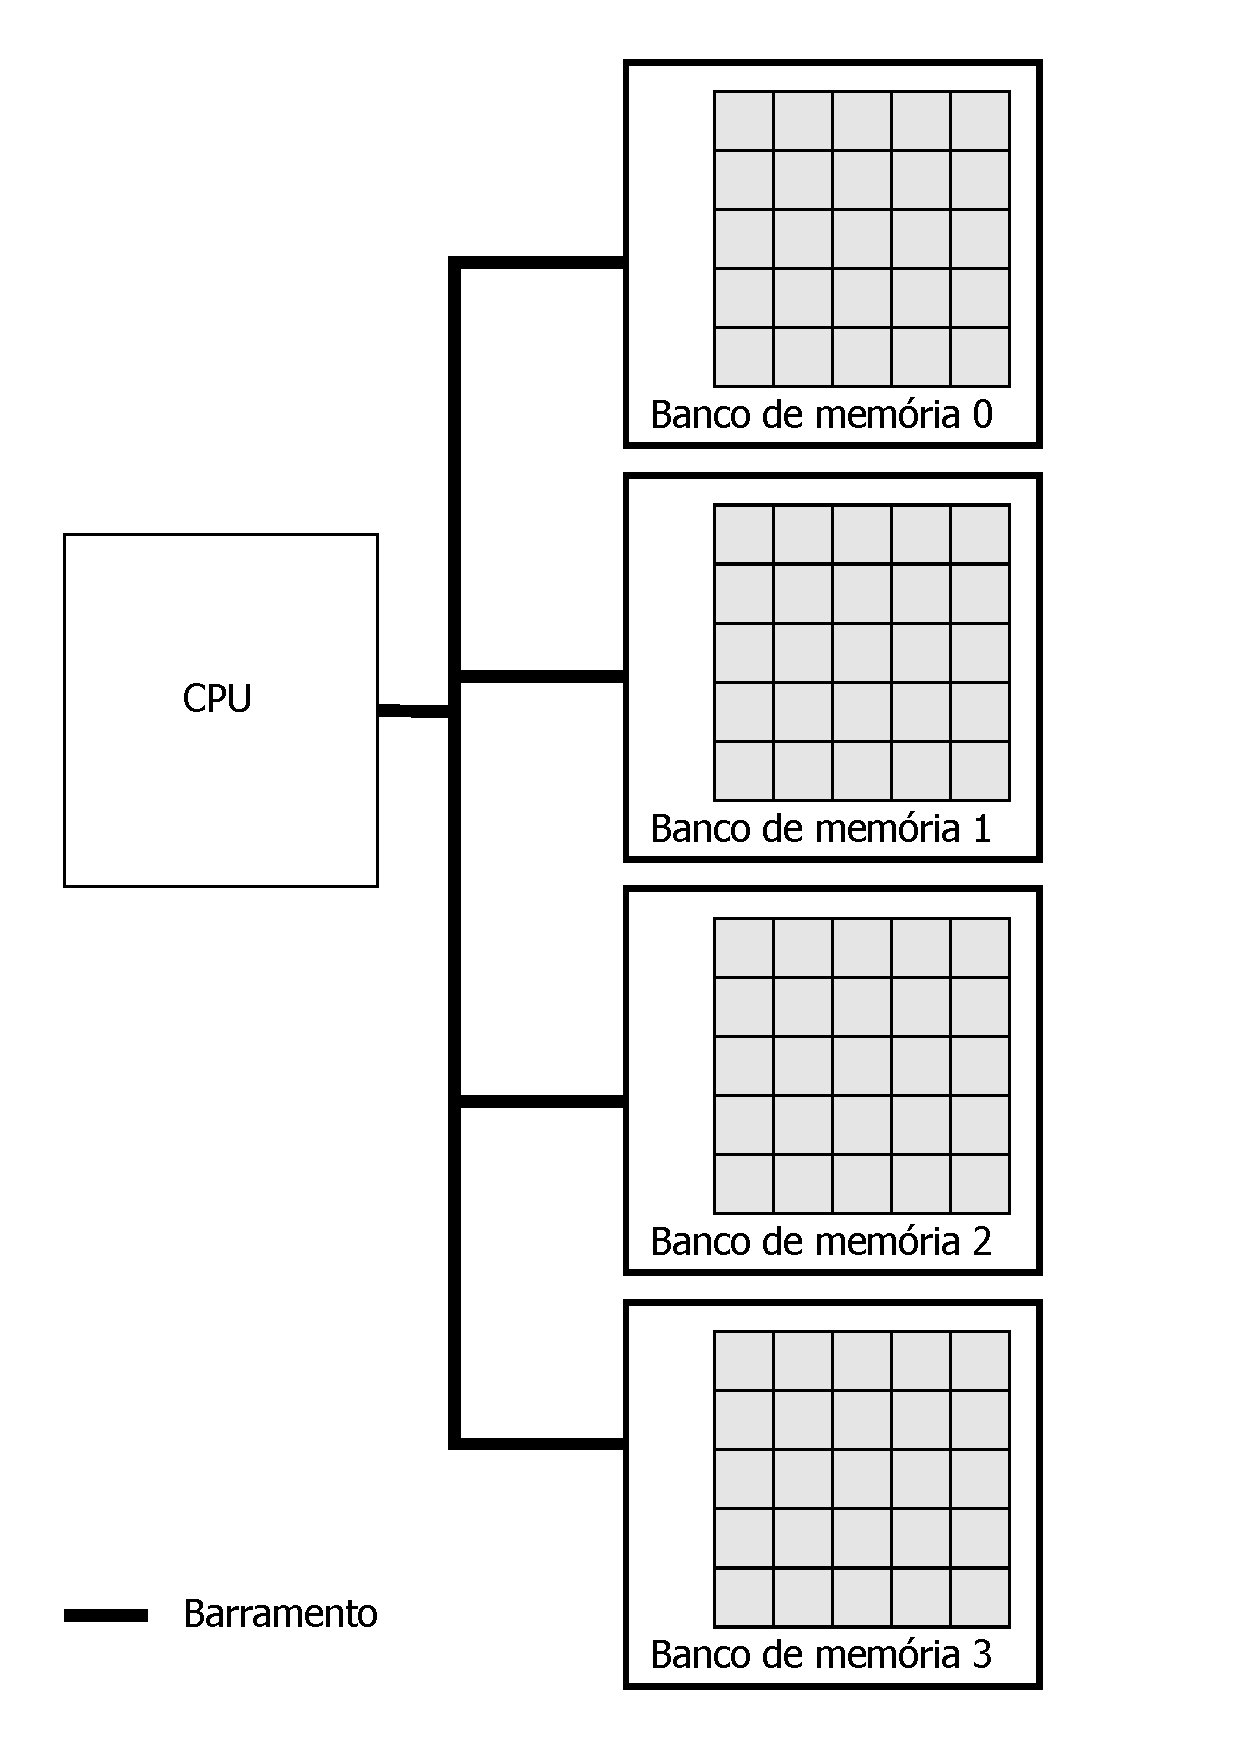
\includegraphics[width = 0.4 \linewidth]{figs/topologia.pdf}}
\subfigure[\label{FIG:MEM_VECTOR}]{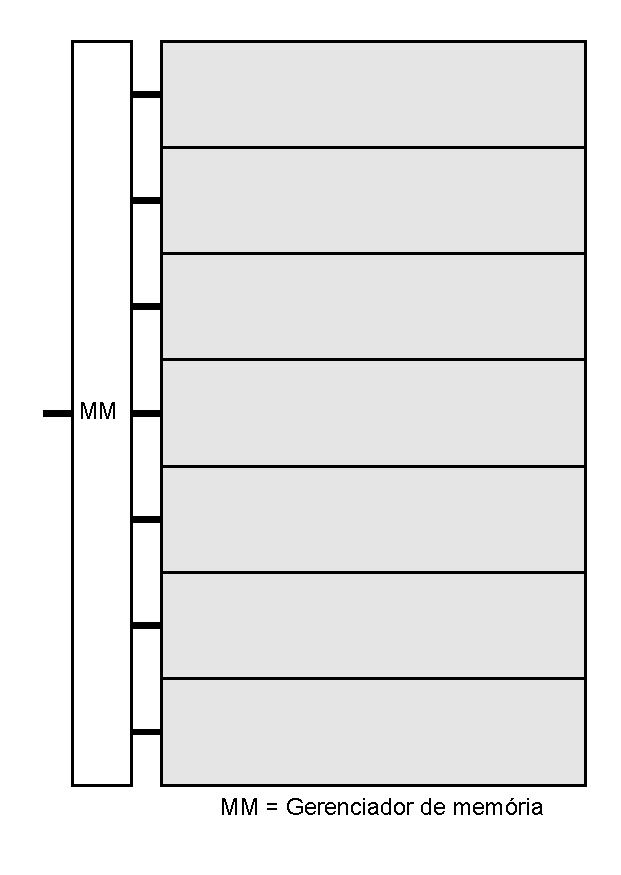
\includegraphics[width = 0.4 \linewidth]{figs/vector.pdf}}
\caption[Topologias da mem�ria]{Topologia da mem�ria como fisicamente disposta (a) e como vista por uma aplica��o (b).} \label{FIG:MEM_TOPOLOGY}
\end{figure}

Al�m disto, por��es fragmentadas da mem�ria f�sica podem ser alocadas para um processo, mas o gerenciador virtualiza estes fragmentos em um espa�o cont�nuo de endere�amento, como ilustrado na Figura \ref{FIG:MEM_VIRTUAL}.

\begin{figure}[!ht]
\centering
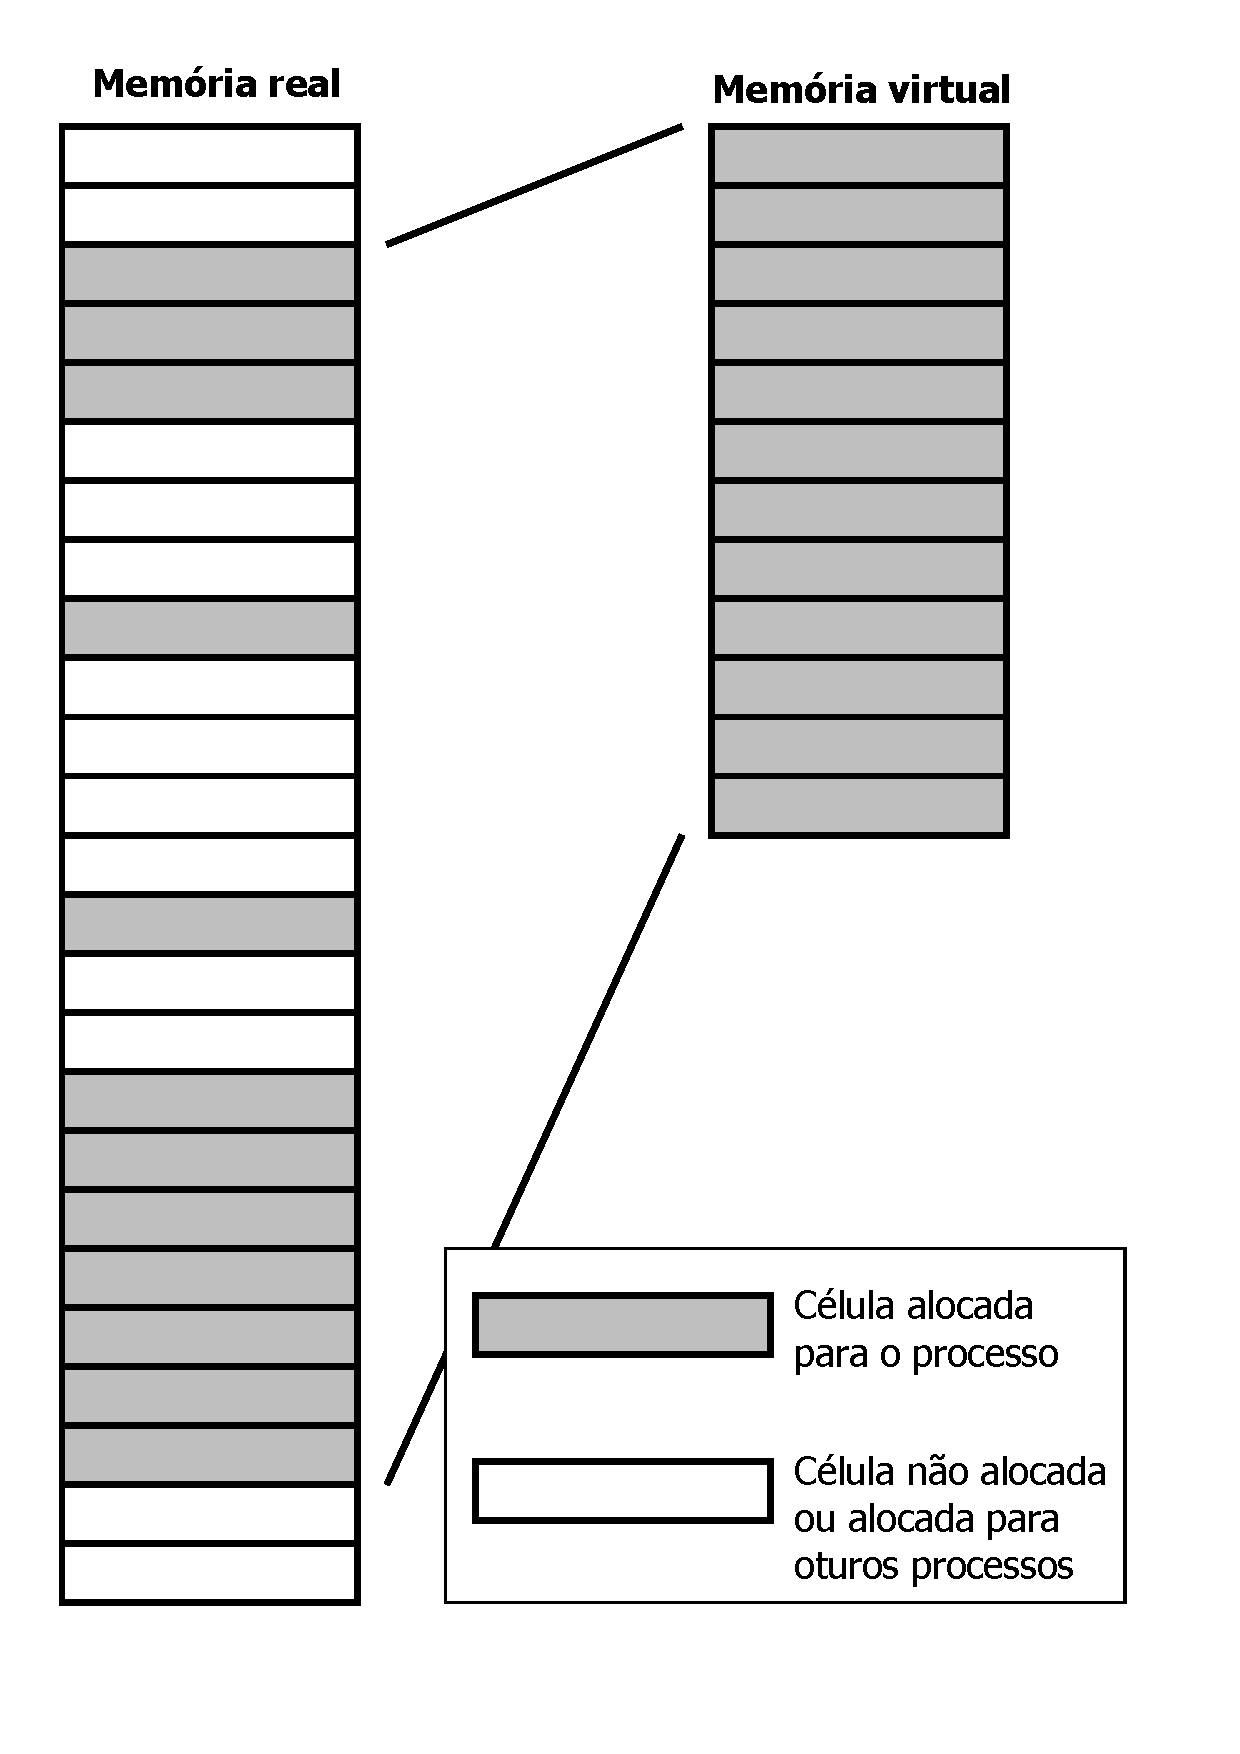
\includegraphics[width = 0.5 \linewidth]{figs/mem_virtual.pdf}
\caption[Mem�ria virtual]{Mem�ria virtual como alocada para um processo (adaptado de \cite{TANENBAUM:2001}).} \label{FIG:MEM_VIRTUAL}
\end{figure}

A pagina��o � outro mecanismo presente nos gerenciadores e est� geralmente associado � mem�ria virtual. Isto faz com que o sistema guarde por��es de dados (p�ginas) da mem�ria principal em uma mem�ria secund�ria, recuperando-as posteriormente quando seu uso for solicitado. Desta forma, o sistema expande a mem�ria virtual dispon�vel para as aplica��es. Geralmente se utiliza como mem�ria secund�ria um espa�o reservado no disco (HD, SSD, etc). Estes dispositivos s�o mais lentos que as \ac{RAM}s mas possuem maior disponibilidade de armazenamento e s�o mais baratos, se levado em conta o valor por byte. \cite{TANENBAUM:2001}

No Linux, o espa�o reservado para pagina��o � chamado de \emph{swap} e pode estar presente ou n�o em um sistema, assim como pode ser habilitado, desabilitado ou redimensionado em tempo de execu��o.

Como o processo de salvar e recuperar as p�ginas do disco � lento, o Linux evita utilizar a �rea de \emph{swap} at� que a disponibilidade de mem�ria livre esteja baixa.

\subsection{Escassez de Mem�ria}

A \ac{OOM} � um estado de um sistema computacional, geralmente indesejado, onde nenhuma mem�ria adicional pode ser alocada para uso pelos programas ou pelo pr�prio sistema operacional.

No caso do Linux, para lidar com este tipo de situa��o � utilizada uma ferramenta, parte do subsitema \ac{LinuxMM}, chamada de OOM \emph{Killer}, que consiste em uma tarefa que sacrifica um ou mais processos para liberar mem�ria para o sistema \cite{OOMKILLER:2009}.

Programas que utilizam muita mem�ria podem esgotar a mem�ria do sistema, fazendo-o deixar de funcionar. Isto pode, por exemplo, levar a uma situa��o em que h� t�o pouca mem�ria que o kernel n�o pode alocar mem�ria para executar uma oper��o de libera��o de mem�ria. Ent�o, neste caso, o OOM Killer � acionado e identifica os processos a serem sacrificados para beneficiar o resto do sistema.

O OOM Killer usa um esquema de pontua��o para decidir qual ou quais processos sacrificar. Os pontos s�o dados pela fun��o \emph{badness}, que utiliza uma f�rmula relativamente simples, documentada no pr�prio c�digo. As regras para gerar a pontua��o s�o:

\begin{itemize}
  \item perder o m�nimo de trabalho realizado;
  \item recuperar a maior quantidade de mem�ria;
  \item n�o matar (\emph{kill}) nada que tenha utilizado pouca mem�ria;
  \item matar o m�nimo de processos (de prefer�ncia apenas um);
  \item tentar matar o processo que o usu�rio espera que v� ser morto (menor surpresa).
\end{itemize}

\subsection{Cache de Mem�ria}

Uma caracter�stica do \ac{LinuxMM} do mecanismo de \emph{cache} de mem�ria. Ele � manipulado pelo Linux Page Cache e funciona da seguinte forma: no Linux, quando um arquivo � acessado, seu conte�do � copiado para a mem�ria para ser trabalhado (lido e/ou escrito); ent�o, quando o processo termina, o \emph{kernel} pode liberar aquela mem�ria ou mant�-la em \emph{cache} para caso algum outro processo o acesse. O mesmo ocorre com algumas outras formas de aloca��o da mem�ria.

Devido ao \emph{cache} em sistemas Linux, ap�s algum tempo de execu��o de processos, apenas uma pequena por��o da mem�ria pode permanecer marcada realmente como livre. A maior parte est� sempre preenchida com conte�do �til, mas nem sempre isso significa que esteja sendo utilizada. Por outro lado h� um ganho de desempenho consider�vel ao acessar recursos recentemente utilizados (em \emph{cache}).

Um conte�do que esteja em \emph{cache} pode ser liberado quando h� uma solicita��o por aloca��o de mem�ria e n�o h� mem�ria livre para atender. Neste caso, o conte�do do \emph{cache} � descartado e a mem�ria � cedida ao processo que solitou a aloca��o. 

\section{Resumo do Cap�tulo}

Este cap�tulo apresentou, de maneira resumida, alguns fundamentos da �rea de testes de mem�ria que s�o �teis para melhor compreens�o deste trabalho, mostrou os v�rios tipos de falhas e testes estudados, dando �nfase nas falhas mais comuns e nos testes de complexidade realiz�vel na tecnologia atual. Tamb�m foram apresentadas algumas caracter�sticas de como o Linux gerencia a mem�ria f�sica do sistema.

No cap�tulo seguinte, ser�o apresentadas as ferramentas utilizadas para o desenvolvimento, teste e valida��o, al�m de detalhes da implementa��o da ferramenta concebida neste trabalho. 
%%%% CAP\'{I}TULO 3: Metodologia
\chapter{Metodologia}
\label{CHP:MET}

Neste cap�tulo s�o descritos os ambientes utilizados no desenvolvimento, avalia��o e teste da ferramenta proposta, chamada de MDiag. Algumas caracter�sticas importantes da implementa��o, que garantem a efic�cia do diagn�stico, s�o apresentadas na Se��o \ref{SEC:DES}. Um sistema autom�tico de inser��o de falhas desenvolvido para valida��o do MDiag atrav�s de simula��o, � detalhado na Se��o \ref{SEC:SIM}. Por fim, � descrito o procedimento de testes em ambientes reais.

    %%% Se��o 3.1:
    \section{Ambiente de Desenvolvimento e Teste}

Para o desenvolvimento deste trabalho, foram utilizados diversos tipos de computadores a fim de garantir compatibilidade com a maior variedade poss�vel de plataformas. Sistemas variando desde kit de desenvolvimento de sistema embarcado at� servidores de grande porte com distribui��es Linux variadas. Todas as m�quinas utilizadas, com exce��o de um computador pessoal do autor, fazem parte do acervo do \ac{LESC} da \ac{UFC}.

Nenhum tipo de bibliotecas, al�m das padr�es do Linux, foram necess�rias durante o desenvolvimento, pois, para favorecer a portabilidade, a ferramenta utiliza apenas funcionalidades presentes no pr�prio \emph{kernel} do Linux, a partir da vers�o 2.6.9.

Para simular as falhas em mem�ria, foi utilizada uma abordagem baseada em \cite{PETRU:2002} (descrita com detalhes na se��o \ref{SEC:SIM}). Um \emph{software} de \emph{debug} com capacidade de estabelecer \emph{breakpoints} em n�vel de \emph{hardware} foi utilizado para interromper a execu��o do teste no momento desejado e escrever um valor de erro na mem�ria, simulando qualquer tipo de falha. O \emph{software} utilizado foi o \ac{GDB}, uma das mais consagradas ferramentas de \emph{debug} para Linux.

Foram realizados testes com mem�rias defeituosas reais e os resultados foram comparados aqueles obtidos por outras ferramentas de diagn�stico do mercado. Os componentes e o procedimento desta avalia��o s�o detalhados na Se��o \ref{SEC:REAL} 
    %%% Se��o 3.2:
    \section{Implementa��o do MDiag}
\label{SEC:DES}

Para o desenvolvimento de um diagn�stico que atua sobre um sistema operacional, alguns cuidados precisam ser tomados para garantir a efic�cia dos testes. Como visto na Se��o \ref{SEC:LINUXMM}, cada acesso � mem�ria passa por uma s�rie de abstra��es at� chegar ao \emph{hardware}. Isto pode acarretar falsos resultados ou inefici�ncias no diagn�stico.

Por exemplo, durante o teste o \emph{kernel} pode guardar parte da mem�ria alocada no \emph{swap}, enquanto o restante � testado. Depois, essas p�ginas podem ser recuperadas e a parte testada pode ser armazenada. A por��o resgatada pode estar em qualquer lugar do espa�o f�sico destinado ao processo, at� mesmo no lugar da por��o que j� foi testada, causando uma dupla checagem nestas c�lulas e deixando de testar outras.

Por isso o MDiag executa uma s�rie de procedimentos, mostrados na Figura \ref{FIG:FLUXO}, antes de executar os algoritmos de teste. O conjunto de opera��es desde a limpeza do \emph{cache} at� a aloca��o, de fato, da mem�ria � um mecanismo projetado neste trabalho chamado de pol�tica de aloca��o de mem�ria do MDiag, que visa maximizar quantidade de mem�ria coberta pelo diagn�stico sem comprometer estabilidade do sistema.

\begin{figure}[!ht]
\centering
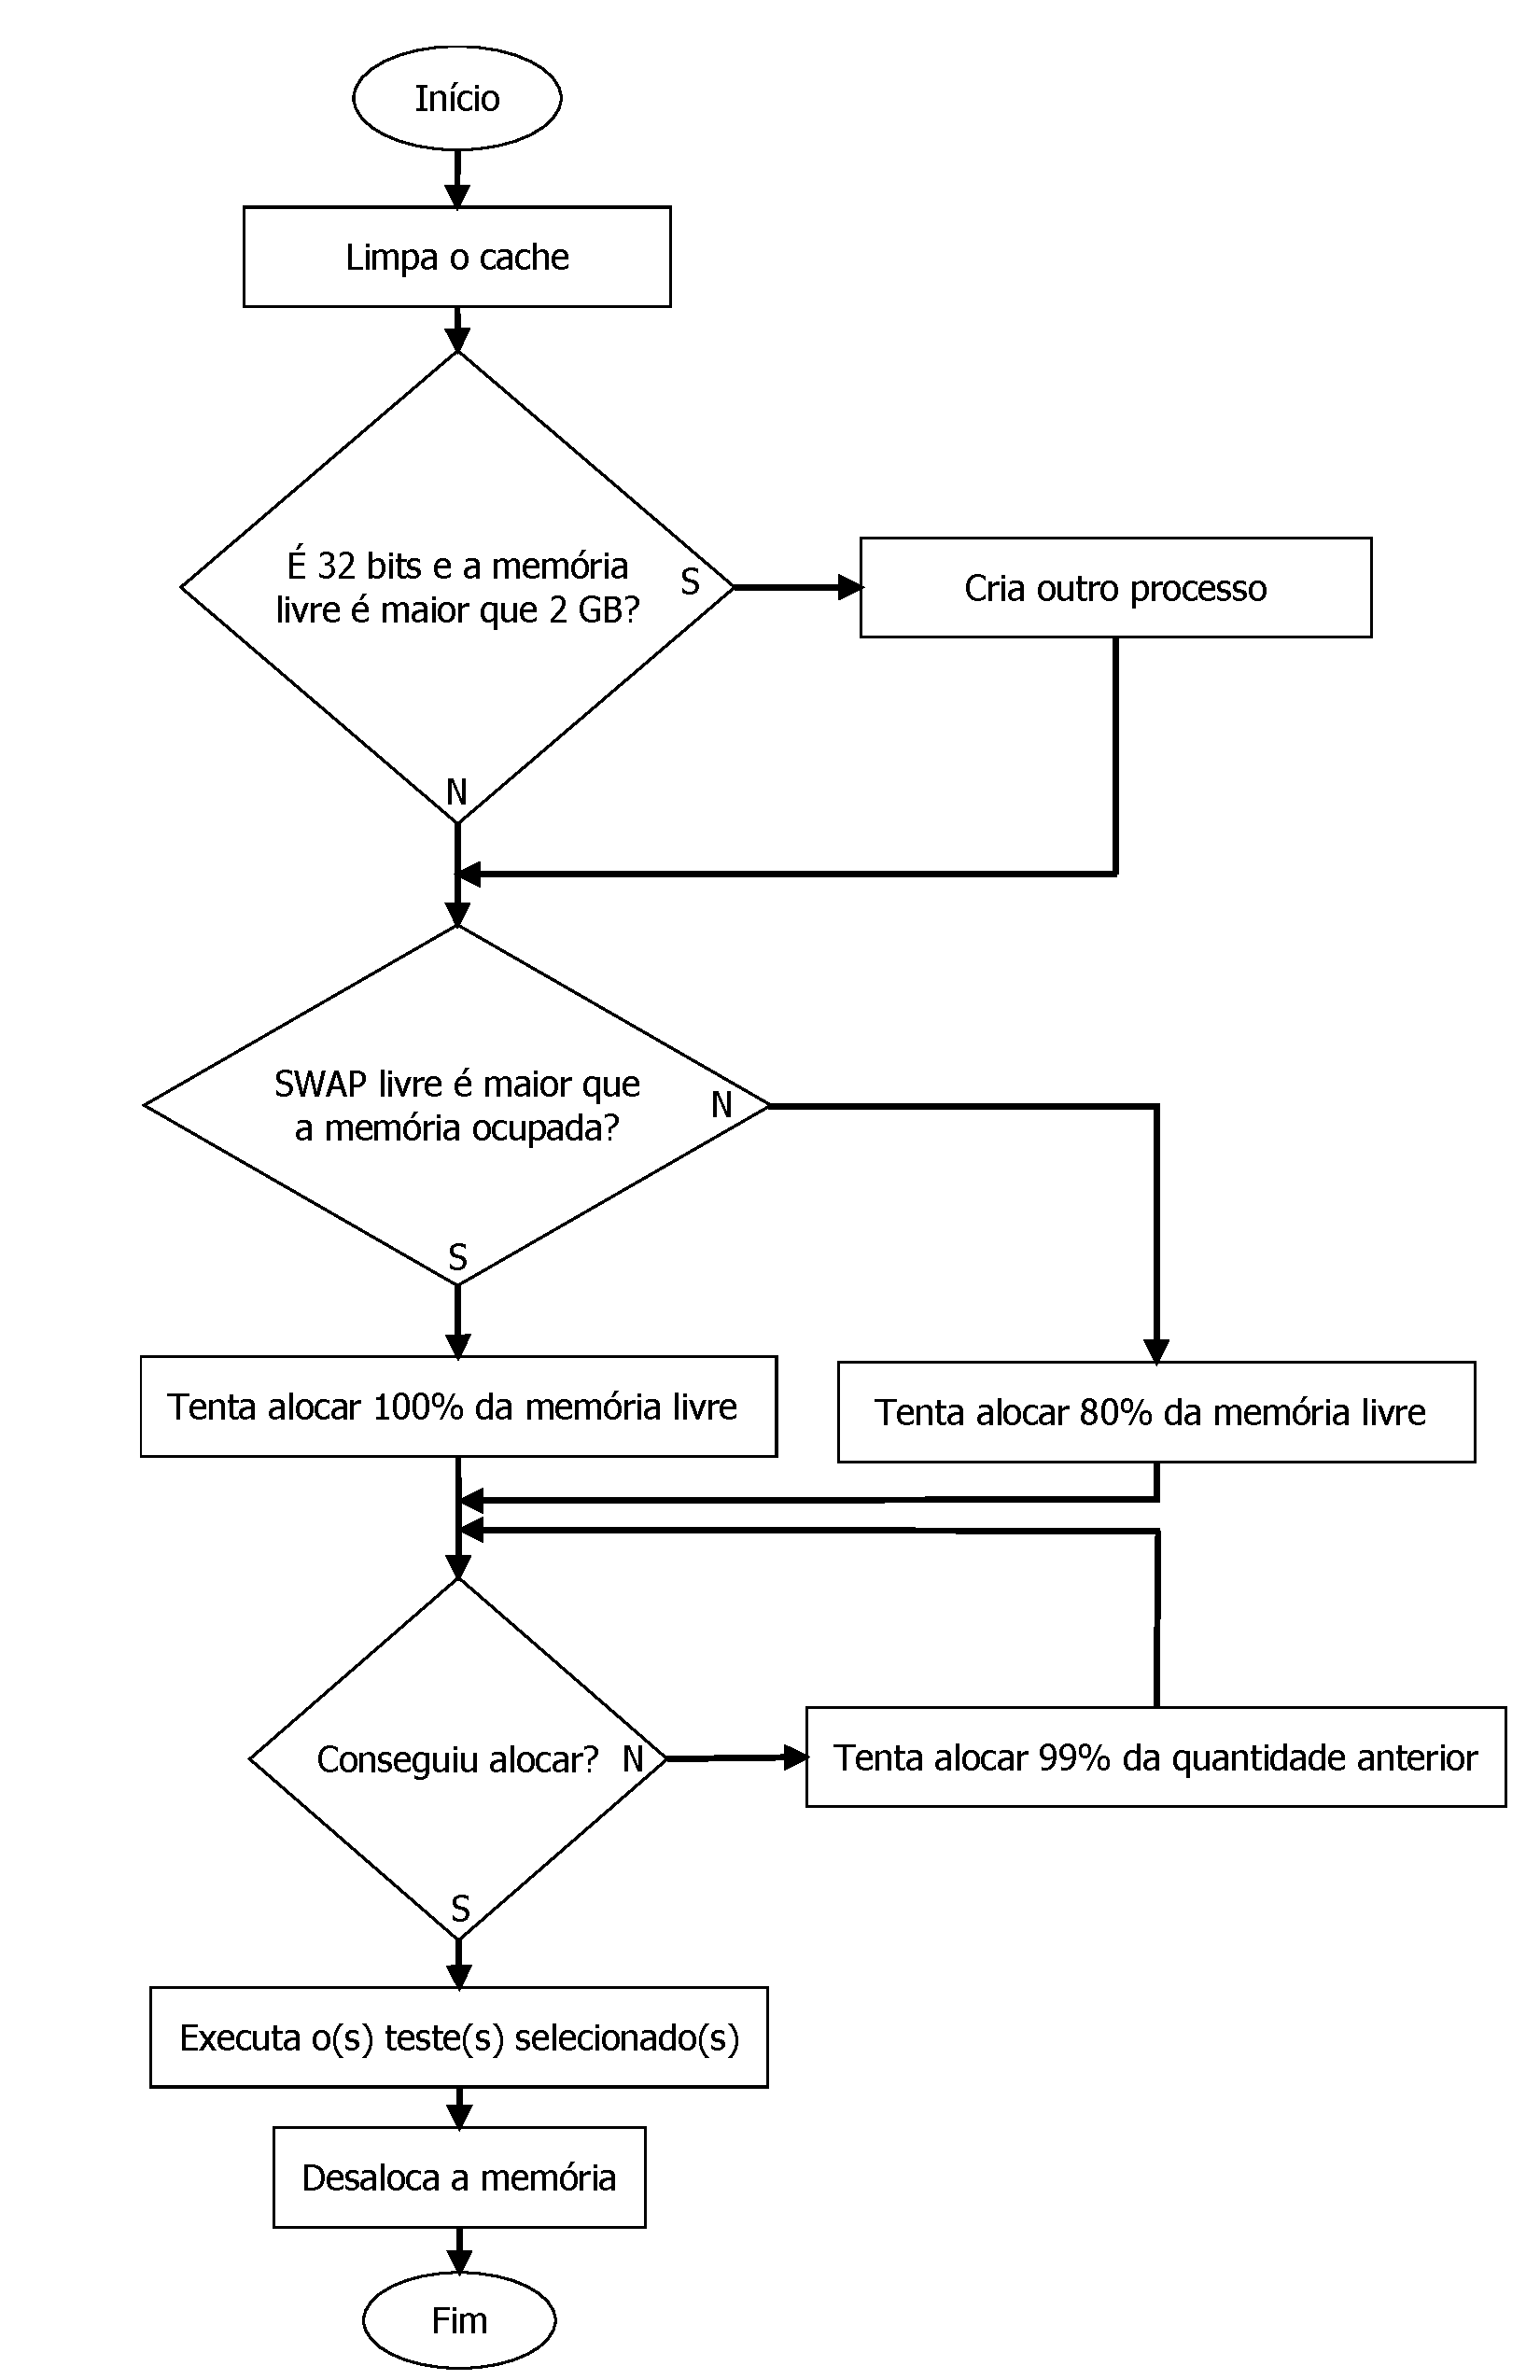
\includegraphics[width = 0.9 \linewidth]{figs/fluxo.pdf}
\caption[Fluxo de execu��o do MDiag]{Fluxo de execu��o do MDiag.} \label{FIG:FLUXO}
\end{figure}

\subsection{Pol�tica de aloca��o de mem�ria}

� imposs�vel que um diagn�stico implementado como um aplicativo, que executa sobre um Linux sem altera��es nos mecanismos de prote��o do \emph{kernel}, possa testar toda a mem�ria instalada, isto porque certa quantidade de mem�ria, chamada de �rea do sistema, � reservada para o pr�prio \ac{SO} guardar suas estruturas de dados, executar e gerenciar as aplica��es. Muitas outras aplica��es executando em paralelo consomem outras por��es da �rea restante. No entanto, quanto mais mem�ria for testada, mais efetivo o diagn�stico ser�, possibilitando detectar mais falhas. Por isso a pol�tica de aloca��o foi tratada com bastante crit�rio durante este projeto.

O Linux possui, simplificadamente, tr�s estados de mem�ria: alocada, em \emph{cache} e livre. O mecanismo de \emph{cache} foi explicado na Se��o \ref{SEC:LINUXMM}. Como foi dito, ap�s algum tempo em opera��o a tend�ncia � que apenas uma pequena parte da mem�ria permane�a realmente livre, a maior parte estar� sendo utilizada como \emph{cache} ou alocada para algum processo. O MDiag aloca apenas a por��o livre da mem�ria, para evitar que o sistema sofra de \ac{OOM}. Por isso o primeiro passo � a limpeza do \emph{cache}, liberando qualquer parte dispens�vel da mem�ria e, consequentemente, aumentando a �rea testada.

Em seguida h� o tratamento de uma limita��o de sistemas 32 bits. Nestes sistemas o endere�amento m�ximo acess�vel por um processo � de 4 GB. O Linux possui um mecanismo chamado \emph{HighMemory} que permite que um \emph{kernel} 32 bits acesse mais de 4 GB de mem�ria f�sica em um \emph{hardware} 64 bits. No entanto, isto permite apenas que mais processos sejam alocados por vez, mas cada um deles ainda ter� acesso a, no m�ximo, 4 GB de mem�ria. Al�m disto, dentro deste espa�o h� uma �rea reservada para que o \emph{kernel} controle aquele processo, al�m de �reas utilizadas como mem�ria de c�digo e pilha. Assim, o m�ximo que uma aplica��o consegue alocar para uso pr�prio varia tipicamente em torno de 3 GB.

Para contornar esta limita��o, o MDiag verifica se o sistema � 32 bits e se a mem�ria livre � maior que 2 GB. Neste caso, o programa se duplica em dois processos id�nticos, mas totalmente independentes (\emph{fork}). Isto faz com que dois testes com os mesmos par�metros sejam executados simultaneamente, cada um fazendo sua pr�pria tentativa de aloca��o e ampliando a mem�ria total testada. � claro que ainda assim pode acontecer de nem toda a mem�ria livre ser alocada, mas o limite � dobrado para aproximadamente $6 GB$.

A aloca��o de mem�ria no MDiag � um processo de duas etapas. Primeiramente h� a aloca��o em si (\emph{malloc}), isto �, solicitar ao \emph{kernel} uma por��o de mem�ria de tamanho fixo para ser utilizada pela aplica��o. Uma vez concedida, esta regi�o deve ser travada (\emph{mlock}). Isto significa que o processo indica ao \emph{kernel} que aquela regi�o de mem�ria n�o pode ser armazenada em \emph{swap}, garantindo que tudo o que foi alocado esteja realmente na mem�ria f�sica da m�quina. Se uma das etapas receber resposta negativa do \emph{kernel}, o processo de aloca��o falhou. Neste caso, � feita uma nova tentativa de aloca��o   com 99\% da quantidade pretendida anteriormente. Este processo se repete at� que se obtenha sucesso ou at� que a quantidade pretendida se torne abaixo de 10 MB.

Outra medida tomada, na pol�tica de aloca��o, para evitar \ac{OOM} � de n�o alocar toda a mem�ria virtual do sistema. Isto � feito assegurando-se de que h� espa�o suficiente no \emph{swap} para armazenar toda a mem�ria atualmente em uso, se necess�rio. Caso contr�rio, apenas 80\% da mem�ria livre � alocada. Este n�mero foi alcan�ado de forma emp�rica com testes em diversas m�quinas reais com diferentes distribui��es Linux, diferentes tamanhos de mem�ria e diferentes perfis de uso (muitos processos ou poucos processos). � o maior percentual em que se notou um baix�ssimo risco de \ac{OOM}.

Ap�s passar por toda a pol�tica de aloca��o, finalmente os testes podem ser aplicados sequencialmente � regi�o de mem�ria alocada.

\subsection{Algor�tmos Implementados}

Neste trabalho foram utilizados seis algoritmos, permitindo realizar testes mais r�pidos ou testes com maior cobertura de falhas. Foram escolhidos os algoritmos de maior reconhecimento na literatura, citados em praticamente todos os artigos e livros da �rea, com uso consagrado na ind�stria e com resultados comprovados em an�lises comparativas de testes de mem�ria \cite{RIEDEL:1995,RAGHURAMAN:2005}.

\subsubsection{March C-}

O March C- � um teste ainda muito utilizado por possuir duas caracter�sticas bastante fortes: entre os testes do tipo marchante, � um dos que possui maior cobertura de falhas; � um teste r�pido, com complexidade de apenas $10 N$ opera��es.

No MDiag foi implementada tamb�m a varia��o proposta por \cite{ADAMS:2003}, chamada de Enhanced March C- e descrita na tabela \ref{TAB:EMARCHC-}. Esta forma melhorada do March C- � mais lenta, com $8N$ opera��es a mais, mas possui uma cobertura de falhas um pouco maior.

As descri��es destes testes j� foram apresentadas na se��o \ref{SEC:TESTES}, especialmente nas Tabelas \ref{TAB:MARCHC-} e \ref{TAB:EMARCHC-}.

\subsubsection{March G}

Da s�rie de testes March, o que obteve melhores resultados at� hoje foi proposto por \cite{VANDEGOOR:1998}. O March G (tabela \ref{TAB:MARCHG}) introduz um novo tipo de elemento al�m das escritas e leitura convencionais. � uma pausa entre as sequ�ncias, que possibilita a detec��o de falha de reten��o (\emph{data retention fault}).

\begin{table}[!ht]
\caption{\emph{March G pattern.}}
\centering
\label{TAB:MARCHG}
\begin{tabular}{| c | l r |}
\hline
1 & W0 & $\Updownarrow$ \\
2 & R0, W1, R1, W0, R0, W1 & $\Uparrow$ \\
3 & R1, W0, W1 & $\Uparrow$ \\
4 & R1, W0, W1, W0 & $\Downarrow$ \\
5 & R0, W1, W0 & $\Downarrow$ \\
6 & pausa & \\
7 & R0, W1, R1 & $\Updownarrow$ \\
8 & pausa & \\
9 & R1, W0, R0 & $\Updownarrow$ \\
\hline
\end{tabular}
\end{table}

\subsubsection{Papachristou}

Para um teste mais completo, o algoritmo adotado foi o proposto por \cite{PAPACHRISTOU:1985}. � um teste longo, que demanda $38N+24N\log_2(N)$ opera��es, o equivalente a $16,9$ minutos para testar 1 GB ou mais de uma hora para testar 4 GB de mem�ria nas condi��es da tabela \ref{TAB:TEMPOS}. Apesar de ser um padr�o antigo, sua abrang�ncia na detec��o de falhas vem sendo confirmada por trabalhos mais recentes \cite{RIEDEL:1995} \cite{PETRU:2002}.

No MDiag, foram implementados os algoritmos parcial e completo de Papachristou. Ambas as varia��es foram apresentados na Se��o \ref{SEC:TESTES}.

Todos os algoritmos at� aqui foram implementados tomando como c�lulas os bytes da mem�ria, portanto cada c�lula possui 8 bits de tamanho. Os estados 0 e 1 em que a c�lula pode estar representam um padr�o qualquer de $00_h$ a $FF_h$ e seu inverso (complemento bit-a-bit), permitindo que os testes detectem erros mais variados. Por exemplo, o March C- � capaz de detectar \emph{idempotent} \ac{CF} se utilizado o estado 0 como o valor $00_h$ e, por consequ�ncia, estado 1 como o valor $FF_h $, mas n�o � capaz de detectar \emph{inversion} \ac{CF}. J� com a utiliza��o do padr�o $55_h$ como o estado 0 e seu inverso $AA_h$ como estado 1, ocorre exatamente o oposto.

\subsubsection{MT}

O mais recente dentre os algoritmos implementados � o MT (Tabela \ref{TAB:MT}). � um teste que possui uma cobertura t�o boa quanto Papachristou, mas de complexidade $O(N)$.

Como visto em sua descri��o na Se��o \ref{SEC:TESTES}, este teste trabalha com base na disposi��o matricial das c�lulas da mem�ria. Desta forma, sua implementa��o foi um pouco diferente dos demais. Primeiramente, para manter a estrutura matricial pressuposta pelo algoritmo, as c�lulas foram tomadas como sendo os \emph{bits} e n�o mais o \emph{bytes} da mem�ria. Assim, tem-se uma matriz $8 \times N$ de c�lulas, podendo-se aplicar os padr�es de fundo da tabela $I_1$ a $I_6$ da \ref{TAB:MTBACKGROUNDS}. Da mesma forma, devido a utiliza��o de padr�es j� bem definidos no algoritmo, este teste n�o permite escolher o que os estados 0 e 1 significam, mesmo porque as c�lulas agora s�o apenas bits, que s� assumem os valores 0 e 1.

\subsection{Desaloca��o da Mem�ria}

O pr�ximo passo, consiste na desaloca��o de toda a mem�ria. Da mesma forma que a aloca��o, este tamb�m � um processo de duas etapas. Primeiro a mem�ria � destravada, para ent�o ser desassociada do processo.

� importante garantir que a mem�ria seja devidamente desalocada, mesmo no caso do programa ter sua execu��o interrompida, seja pelo usu�rio ou pelo \emph{kernel}. Isto porque a quantidade de mem�ria reservada para o diagn�stico representa uma por��o significativa do total dispon�vel, al�m da regi�o estar travada, n�o podendo nem mesmo ser despejada para \emph{swap}.

O MDiag utiliza um manipulador de sinal (\emph{signal handler}) que nada mais � que uma fun��o a ser executada sempre que o \emph{kernel} enviar certo sinal. Este manipulador monitora um sinal do \emph{kernel} que � disparado sempre que h� uma tentativa de interrup��o ao processo. O manipulador deve ser r�pido, pois o \emph{kernel} envia este sinal como aviso de que o programa ser� fechado, e caso o processamento n�o cesse, o \emph{kernel} poder� matar o processo abruptamente. 
    %%% Se��o 3.3:
    \section{Inser��o de Falhas}
\label{SEC:SIM}

A fim de comprovar a efic�cia dos testes, foi desenvolvido um ambiente de valida��o autom�tico com inser��o de falhas via \emph{debugging}.

O m�todo utiliza elementos de \emph{debugging} presente na maioria dos processadores atuais. O \ac{GDB} foi usado como interface de \emph{software} para explorar esses recursos do \emph{hardware}. Foram utilizadas principalmente duas estruturas: \emph{breakpoint} e \emph{watchpoint}. O primeiro � apenas um ponto de parada na execu��o do programa, congelando-o at� que seja dado o comando para continuar. O segundo � similar ao primeiro, mas o crit�rio de parada n�o est� associado a um ponto espec�fico do c�digo, mas a uma vari�vel, fun��o ou posi��o da mem�ria. A execu��o � interrompida cada vez que houver uma tentativa de leitura ou escrita no endere�o monitorado.

\subsection{Falhas simuladas}

As falhas inseridas foram limitadas aos erros mais desafiadores para os algoritmos de teste de mem�ria, eliminando redund�ncias no sistema e otimizando o tempo de valida��o. Os modelos mais simples, como \ac{SAF} e \ac{TF}, n�o foram levados em considera��o, pois todos os algoritmos apresentados possuem cobertura de 100\% na sua detec��o \cite{RIEDEL:1995} \cite{PETRU:2002} \cite{RAGHURAMAN:2005}. Foram escolhidas apenas falhas representativas, em que � esperado que os testes n�o possam detectar todas as varia��es poss�veis.

Os modelos de falha que apresentam maior dificuldade na detec��o s�o os de acoplamento. Tanto os \ac{CF} simples, como \ac{NPSF} ou, de forma mais geral, falhas de \emph{k-coupling}. Para a valida��o foram inseridas falhas do tipo \emph{idempotent} \ac{CF}, \emph{inversion} \ac{CF} e \emph{3-coupling fault}. Estas foram aplicadas apenas entre c�lulas vizinhas, pois, al�m de ser a situa��o mais comum encontrada em mem�rias reais \cite{PETRU:2002}, cobre as tr�s ordena��es poss�veis de acoplamento: a v�tima (c�lula que sofre transi��o err�nea) acima da agressora (c�lula que dita o estado da v�tima), a v�tima abaixo da agressora e a v�tima e a agressora no mesmo byte.

Da mesma forma, para eliminar redund�ncia no sistema e otimizar o tempo de valida��o, os \emph{bits} utilizados foram limitados aos mais representativos. As falhas se combinam apenas entre os bits 0, 1, 6 e 7 de cada \emph{byte}. Assim os casos cobertos s�o: \emph{bits} nas bordas da c�lula, \emph{bits} fora das bordas, \emph{bits} vizinhos, \emph{bits} distantes, v�tima a direita da agressora e v�tima a esquerda da agressora.

De forma mais simples, cada falha foi inserida com todas as combina��es entre acoplado e acoplador nos bits destacados na figura \ref{FIG:CELULAS_FALHAS}.

\begin{figure}[!ht]
\centering
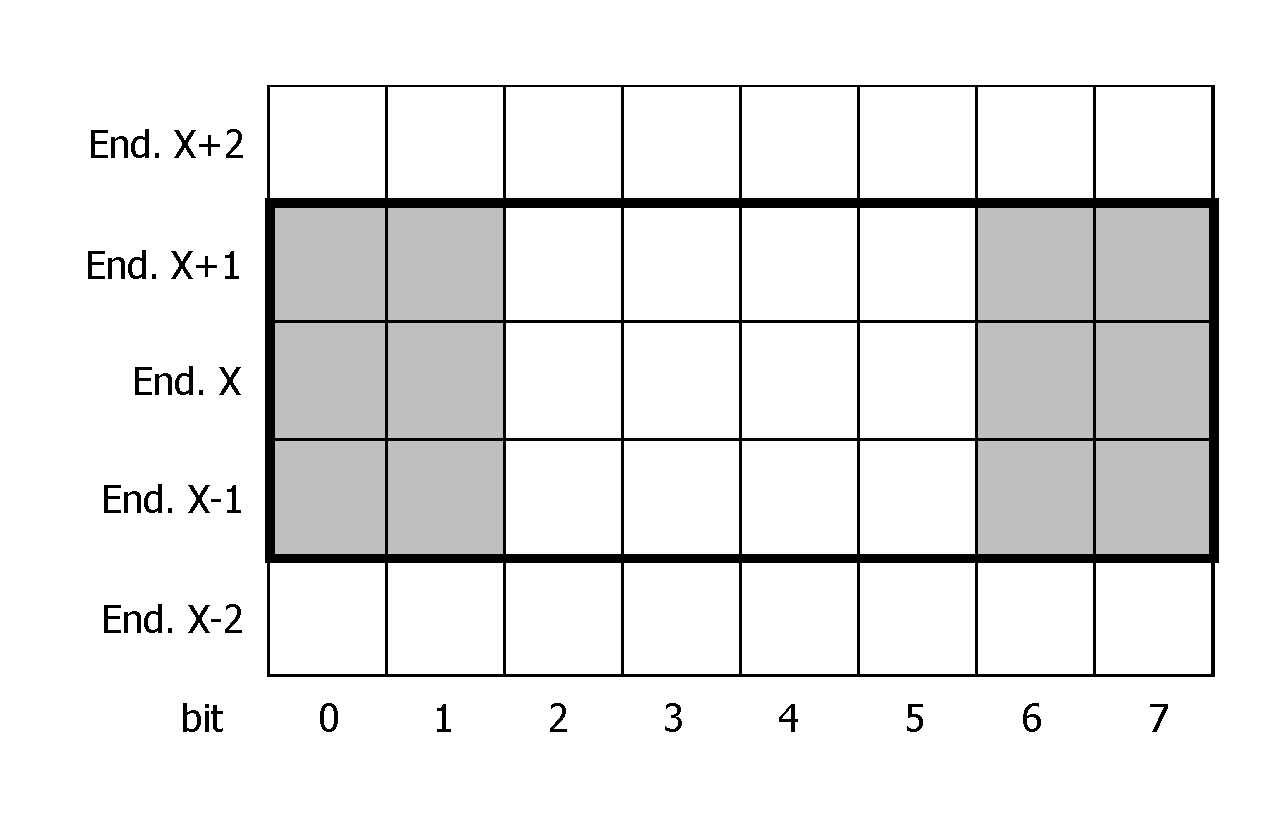
\includegraphics[width = 0.7 \linewidth]{figs/celulas_falhas.pdf}
\caption[Bits atingidos pela inser��o de falhas]{Bits atingidos pela inser��o de falhas.} \label{FIG:CELULAS_FALHAS}
\end{figure}

Para cada modelo simulado, as combina��es poss�veis s�o dadas por: $(b \cdot 3 - 1) \cdot b$ para acoplamento entre duas c�lulas e $(b \cdot 3 - 2) \cdot (b \cdot 3 - 1) \cdot b$ para tr�s, com $b$ sendo a quantidade de \emph{bits} em que as falhas podem ocorrer em  cada \emph{byte}. Para a falha \emph{3-coupling fault} h� duas possibilidades: que a c�lula v�tima sofra transi��o quando uma das outras for escrita e a terceira esteja no estado 0 ou quando esta esteja no estado 1.

Portanto, o total de combina��es de falhas geradas para b = 4 �:

$2 \cdot (4 \cdot 3 - 1) \cdot 4 = 88$

$+$

$2 \cdot (4 \cdot 3 - 2) \cdot (4 \cdot 3 - 1) \cdot 4 = 880$

$= 968$ falhas.

\subsection{Sistema de inser��o de falhas}

A Figura \ref{FIG:FLUXO_SIM} mostra os passos do sistema de inser��o de falhas elaborado para validar o MDiag.

\begin{figure}[!ht]
\centering
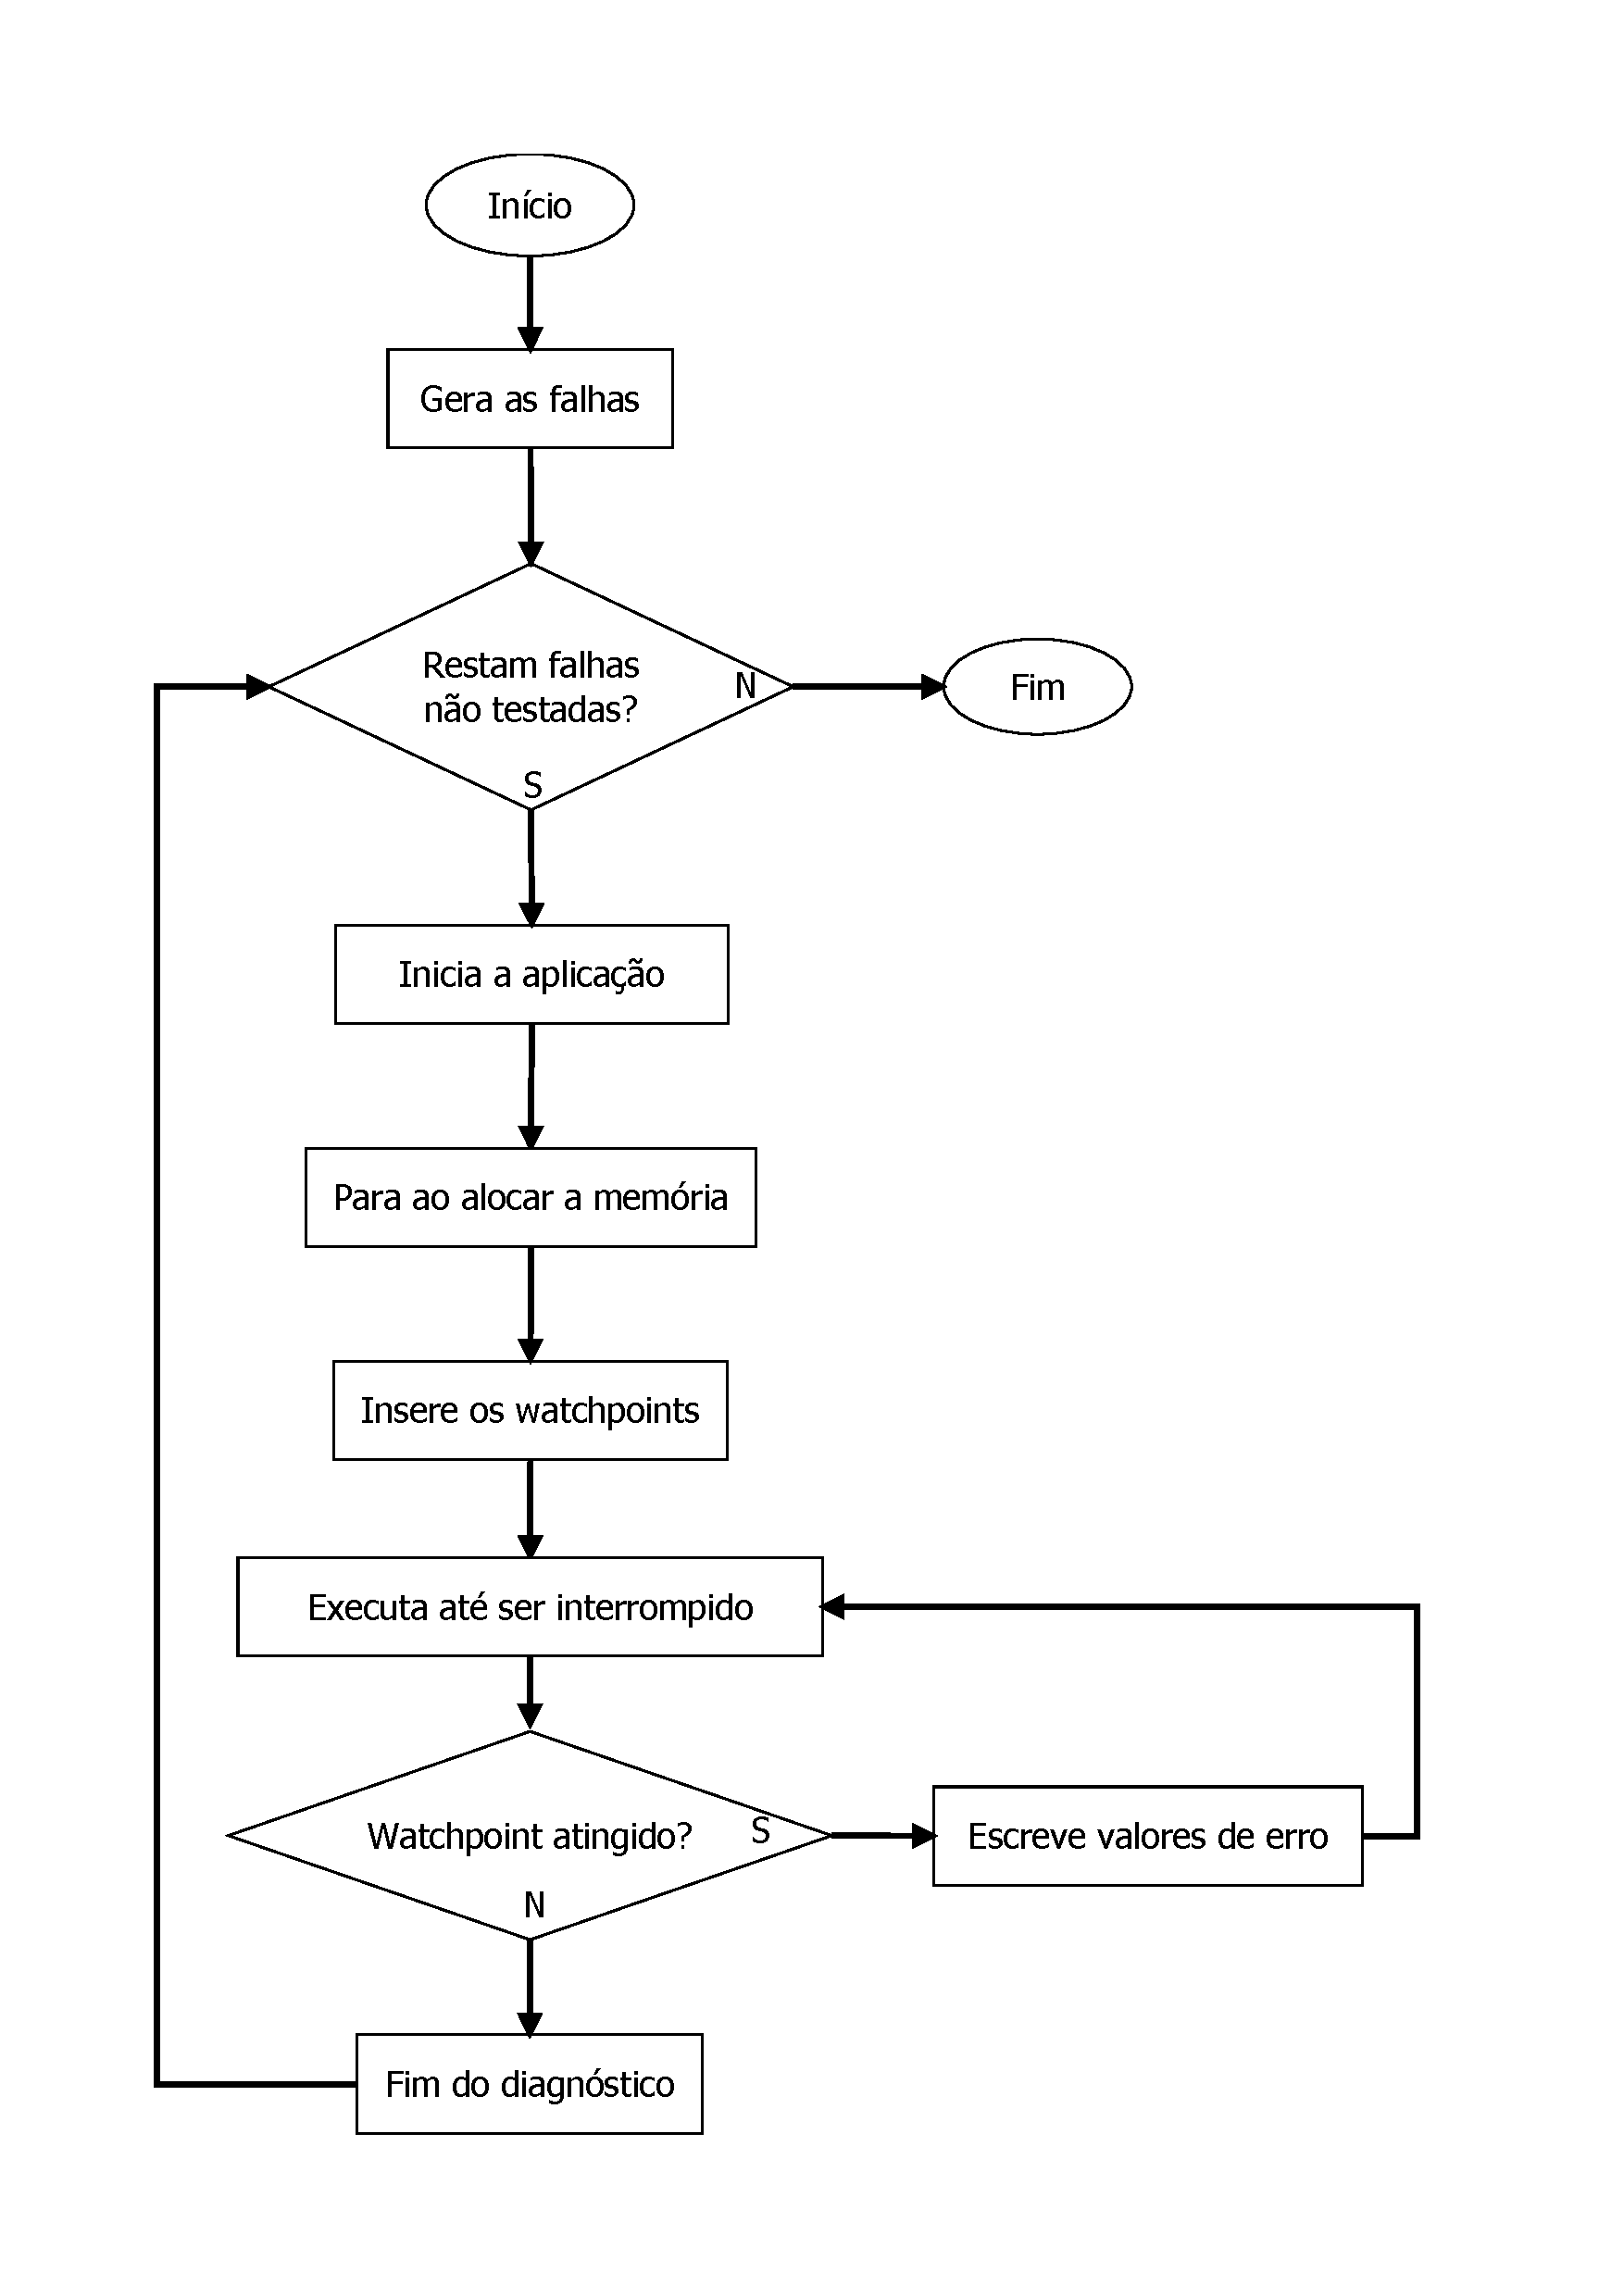
\includegraphics[width = 0.9 \linewidth]{figs/fluxo_sim.pdf}
\caption[Fluxograma do m�todo de inser��o de falhas]{Fluxograma do m�todo de inser��o de falhas.} \label{FIG:FLUXO_SIM}
\end{figure}

As falhas s�o geradas atrav�s de um \emph{script} que escreve arquivos com os modelos das falhas utilizando comandos pr�prios do \ac{GDB}. %Por exemplo, uma falha do tipo \ac{CF} entre o \emph{bit} 3 do endere�o 100 e o \emph{bit} 5 do endere�o 101 � representada por um \emph{script} com os seguintes comandos do \ac{GDB}:

%\begin{quote}
%set \$x = buffer[100] \& ($\sim$(1$\ll$3))
%
%set \$y = ((buffer[101] \& (1$\ll$5)) $\gg$ 5) $\ll$ 3
%
%set buffer[100] = \$x | \$y
%\end{quote}

Para otimizar o tempo de valida��o, as falhas s�o inseridas em conjuntos. A quantidade � limitada pelo m�ximo de \emph{watchpoints} que o processador utilizado suporta. Neste trabalho foi poss�vel inserir tr�s falhas a cada execu��o do ciclo maior da figura \ref{FIG:FLUXO_SIM}. O endere�o de cada uma � gerado a uma dist�ncia de 3 c�lulas da anterior, possibilitando que os arranjos da figura \ref{FIG:CELULAS_FALHAS} n�o se sobreponham. Assim, foram necess�rias 323 itera��es para cobrir todas as falhas testadas. A quantidade de mem�ria necess�ria para comportar $n$ falhas � de $4 \cdot n - 1$. Portanto, apenas 11 bytes s�o suficientes para comportar as falhas inseridas em uma itera��o. Por este motivo, a quantidade de mem�ria alocada pelo MDiag, durante este processo de valida��o, foi for�ada para o m�ximo de 1 MB, diminuindo bastante o tempo de teste de cada algoritmo.

O MDiag foi desenvolvido de modo a guardar em um arquivo de relat�rio todos os acontecimentos relevantes durante a sua execu��o, como a quantidade de mem�ria alocada, tempo de execu��o, falhas encontradas, etc. Estes relat�rios passaram por um tratamento autom�tico posterior para se obter os resultados relevantes. Estes resultados s�o apresentados e discutimos na pr�xima se��o. 
    %%% Se��o 3.4:
    \section{Teste em Ambientes Reais}
\label{SEC:REAL}

Al�m do ambiente de simula��o de falhas descrito na se��o anterior, o MDiag tamb�m foi submetido a situa��es de uso reais a fim de garantir sua utilidade pr�tica.

O acervo utilizado para teste foi composto por dez placas de mem�ria, algumas em perfeito funcionamento, outras com falhas. Metade delas possu�am encapsulamento \ac{SO-DIMM}, pr�prias para computadores de dimens�es reduzidas, como \emph{notebooks} e \emph{netbooks}, e as outras, encapsulamento \ac{DIMM}, geralmente usadas nos computadores pessoais comuns, estilo \emph{desktop}, ou em servidores.

Nesses testes, o MDiag confrontou dois \emph{softwares} de diagn�stico consagrados no mercado. O primeiro foi o \ac{LTT} \cite{LTT:2011}, desenvolvido pela PC-Doctor \cite{PCDOCTOR:2011} para os computadores da fabricante Lenovo. Na realidade este produto re�ne um conjunto de diagn�sticos que cobre quase todos os componentes da m�quina. O segundo foi o Memtest86+ \cite{MEMTEST:2011}, umas das ferramentas de diagn�stico de mem�ria mais abrangentes em termos de cobertura de falhas.

� importante ressaltar que o \ac{LTT} foi utilizado com o sistema operacional Windows, enquanto o Memtest86+ � uma ferramenta \emph{stand-alone} que executa diretamente de uma m�dia externa, como um CD ou \emph{pendrive} sem carregar nenhum \ac{SO}. Estas caracter�sticas influenciaram bastante nos resultados, pois afetam diretamente a quantidade de mem�ria testada.

O teste com cada ferramenta foi executado cinco vezes para cada m�dulo de mem�ria. Estas, por sua vez, foram etiquetadas cegamente, n�o havendo nenhum conhecimento pr�vio sobre a presen�a ou aus�ncia de falhas em cada uma delas.

Uma estimativa do tempo de execu��o de cada algoritmo implementado pelo MDiag foi elaborada com base na sua complexidade e levando em considera��o o \emph{overhead} das opera��es realizadas entre as escritas e leituras. Um algoritmo pode exigir apenas $10 N$ opera��es de acesso a mem�ria, mas para ser realizado ainda � necess�rio alocar mem�ria, executar checagens ap�s as leituras, incrementar o contador de endere�o, desalocar mem�ria, etc. Assim, o total de opera��es de uma implementa��o deve ser maior que o simples valor da complexidade.

A estimativa utilizou a f�rmula \ref{EQU:FUNCLOGIS}, na qual $C$ � a complexidade do algortimo e $O$ � um par�metro de tempo m�dio por opera��o, levando-se em conta alguns processamentos extras necess�rios. O valor de $O$ foi medido para cada algoritmo, individualmente, dividindo-se o tempo gasto para executar um elemento de teste pela quantidade de opera��es naquele elemento.

\begin{equation}
{T_{est} = C \cdot O}
\label{EQU:FUNCLOGIS}
\end{equation}


\section{Resumo do Cap�tulo}

Neste cap�tulo foram descritos os principais passos e medidas tomadas no desenvolvimento da aplica��o.
Tamb�m foi abordada a metodologia de valida��o elaborada para medir a efici�ncia dos algoritmos escolhidos.

No cap�tulo seguinte, s�o apresentados os resultados dos testes de inser��o de falhas utilizados para validar a ferramenta, al�m de medir o desempenho desta em rela��o a ferramentas do mercado.


%%%%%%%%%%%%%%%%%%%%%%%%%%%%%%%%%%%%%%%%%%%%%%%%%%%%%%%%%%%%%%%%%
%%%% CAP\'{I}TULO 4: Resultados
\chapter{Resultados}
\label{CHP:RESULT}

Neste cap�tulo ser�o abordados os resultados adquiridos com os testes realizados a partir da metodologia descrita na se��o \ref{SEC:SIM} e testes comparativos do MDiag com ferramentas existentes em mem�rias reais.

\section{Testes com inser��o de falhas}

O mecanismo de inser��o de falhas apresentado simulou um total de 968 combina��es diferentes de falhas dos tipos \emph{idempotent} \ac{CF}, \emph{inversion} \ac{CF} e \emph{3-coupling fault}. O tempo total de simula��o foi de 88 minutos. A tabela \ref{TAB:FALHAS} mostra a quantidade de falhas detectadas para cada algoritmo.

\begin{table}[!ht]
\caption{Falhas detectadas por algoritmo.}
\centering
\label{TAB:FALHAS}
\begin{tabular}{| c | c | c |}
\hline
Algoritmo & Falhas detectadas & Falhas detectadas (\%) \\
\hline
March C- & 944 & 97,52\% \\
Enhanced March C- & 956 & 98,76\% \\
March G & 956 & 98,76\% \\
Papachritou Parcial & 964 & 99,58\% \\
Papachristou Completo & 964 & 99,58\% \\
MT & 964 & 99,58\% \\
\hline
\end{tabular}
\end{table}

O resultado condiz com o esperado, porque a quantidade de falhas detectadas cresce de acordo com a evolu��o dos algoritmos. Algumas diferen�as de cobertura entre os testes n�o foram percebidas, como entre o Papachristou parcial e completo. Isto � explicado pela pequena variedade de modelos simulados. � de se esperar que, com a amplia��o dessa diversidade, os resultados revelem maior contraste entre os algoritmos.

\section{Testes com Mem�rias Reais}

Os testes comparativos entre o MDiag e ferramentas existentes foram realizados em um conjunto de 10 placas de mem�ria, algumas possuindo falhas, outras n�o. As de n�mero 01 a 05 s�o de encapsulamento \ac{DIMM} e as de 06 a 10, encapsulamento \ac{SO-DIMM}.
Todas as ferramentas foram executadas nas configura��es padr�o, isto significa que todas executaram o teste mais completo, com todos os algortimos implementados por cada uma.

Os resultados est�o sintetizados na tabela \ref{TAB:REAIS}. Cada teste tem tr�s possibilidades de resultado: nenhuma falha encontrada (\checkmark), uma ou mais falhas encontradas (F) ou n�o foi poss�vel executar o teste ($\varnothing$). Esta �ltima significa que a mem�ria n�o passou no \ac{POST}, uma sequ�ncia de testes realizada pelo \ac{BIOS} que verifica preliminarmente se o sistema se encontra em estado operacional. Outra possibilidade � que o \ac{SO} n�o tenha conseguido executar por tempo suficiente para realizar o teste, provavelmente devido ao uso de parte danificada.

\begin{table}[!ht]
\caption{Resultados dos testes em mem�rias reais.}
\centering
\label{TAB:REAIS}
\begin{tabular}{| c | c | c | c |}
\hline
Mem�ria & MDiag & LTT & Memtest86+ \\
\hline
Mem�ria 01 & \checkmark & \checkmark & \checkmark \\
Mem�ria 02 & $\varnothing$ & $\varnothing$ & $\varnothing$ \\
Mem�ria 03 & \checkmark & \checkmark & \checkmark \\
Mem�ria 04 & \checkmark & \checkmark & \checkmark \\
Mem�ria 05 & $\varnothing$ & $\varnothing$ & $\varnothing$ \\
Mem�ria 06 & F & $\varnothing$ & F \\
Mem�ria 07 & \checkmark & \checkmark & \checkmark \\
Mem�ria 08 & $\varnothing$ & $\varnothing$ & F \\
Mem�ria 09 & \checkmark & \checkmark & \checkmark \\
Mem�ria 10 & F & F+$\varnothing$ & F \\
\hline
\end{tabular}
\end{table}

A compara��o mostra coer�ncia de resultados entre as ferramentas. As mem�rias 02 e 05 n�o passaram no \ac{POST}, ent�o n�o puderam ser testadas em nenhuma ferramenta. O Memtest86+, com a vantagem de n�o utilizar \ac{SO}, conseguiu testar todas as outras, detectando tr�s placas com falha. Destas, o MDiag n�o p�de ser executado na de n�mero 08, pois o Linux n�o conseguiu concluir sua inicializa��o, mas as outras tamb�m foram diagnosticadas com falha. Nos testes com o LTT, o Windows entrou em falha cr�tica antes de executar a ferramenta. Apenas em uma das itera��es com a mem�ria 10 foi poss�vel finalizar o teste, obtendo o mesmo resultado que o Memtest86+ e o MDiag.

O MDiag mostrou-se eficaz na detecc�o de falhas reais, com resultados compat�veis com o Memtest86+. Por executar sobre Linux, apresentou, ainda, vantagem em rela��o ao \ac{LTT}, conseguindo testar mem�rias com falhas com maior estabilidade.

\section{Tempo de Execu��o}

Al�m da cobertura de falhas, � importante considerar o tempo de execu��o de cada ferramenta. O LTT executa 11 algoritmos em sequ�ncia, n�o possuindo op��o para selecionar apenas alguns deles. O Memtest86+ possui 12 tipos de testes e permite selecionar quais ser�o executados. O MDiag possui 6 algoritmos, tamb�m permitindo a sele��o de quais ser�o executados. Assim, o LTT demanda um tempo fixo de execu��o para uma dada m�quina, enquanto o Memtest86+ e o MDiag podem ser configurados para testes r�pidos, m�dios ou longos de acordo com os algortimos selecionados.

Foi feita uma estimativa do tempo de execu��o de cada algoritmo implementado pelo MDiag, tomando como base na sua complexidade. O valor foi confrontado com o valor real medido. A estimativa levou em considera��o parte do \emph{overhead} introduzido pelo processamento extra necess�rio entre cada opera��o de escrita/leitura.

A tabela \ref{TAB:TXC} traz as medidas e as estimativas do tempo de execu��o, al�m da express�o da sua complexidade. Os dados da tabela s�o mostrados no gr�fico da figura \ref{FIG:TEMPOS_TESTES}, com exce��o do Papachristou Completo que difere dos demais por duas ordens de grandeza.

\begin{table}[!ht]
\caption{Tempo de execu��o.}
\centering
\label{TAB:TXC}
\begin{tabular}{| c | c | c | c |}
\hline
Algoritmo & Complexidade & Tempo estimado & Tempo medido \\
\hline
March C- & $10 N$ & 56 s & 61 s \\
Enhanced March C- & $18 N$ & 76 s & 84 s \\
March G & $23 N$ & 95 s & 121 s \\
Papachritou Parcial & $38 N$ & 159 s & 181 s \\
Papachristou Completo & $36 N + 24 N \log_2(N)$ & 18934 s & 18032 s \\
MT & $36 N$ & 280 s & 221 s \\
\hline
\end{tabular}
\end{table}

\begin{figure}[!ht]
\centering
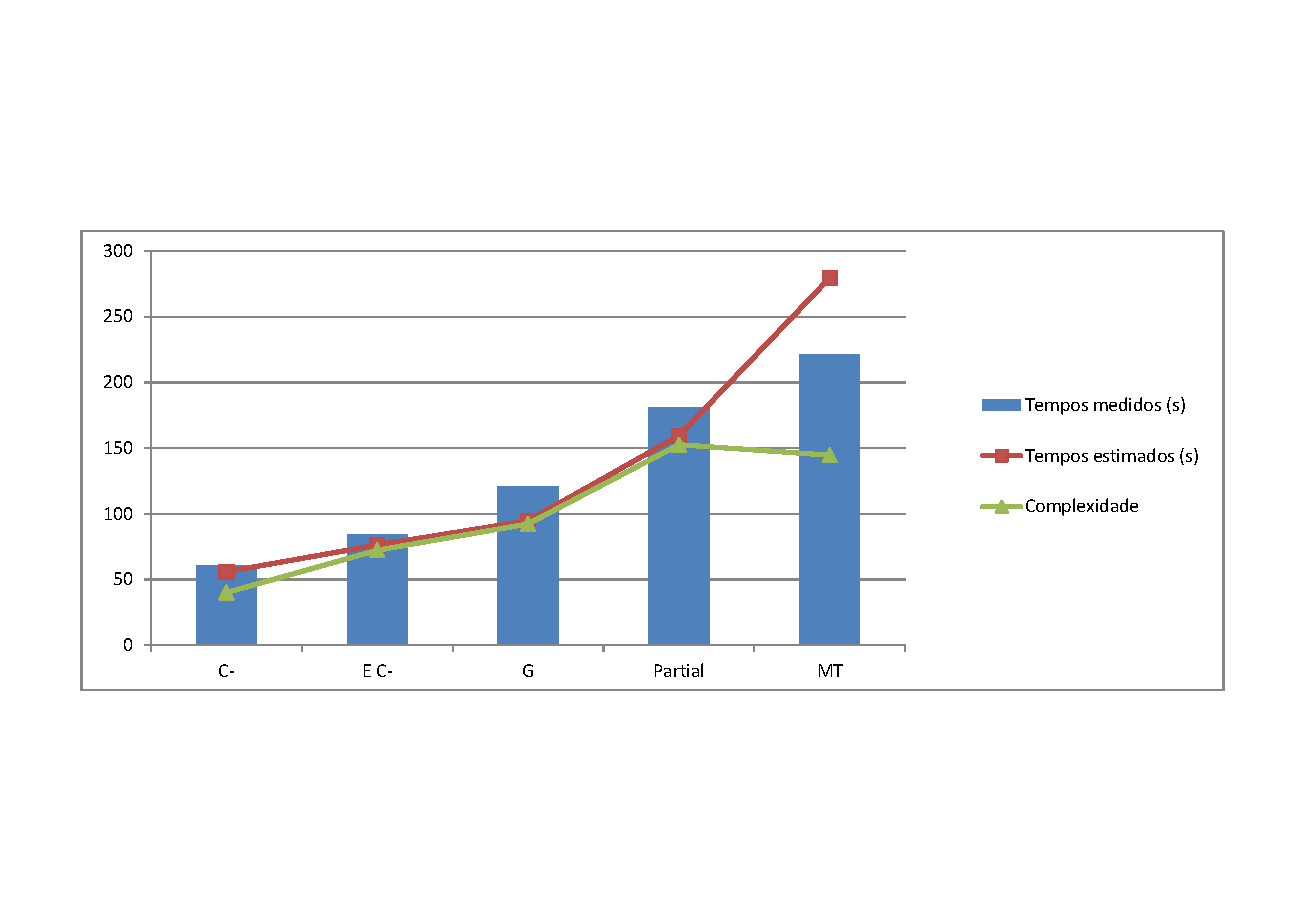
\includegraphics[width = 1 \linewidth]{figs/tempos_testes.pdf}
\caption[Tempo m�dio de execu��o \emph{versus} complexidade]{Tempo m�dio de execu��o \emph{versus} complexidade.} \label{FIG:TEMPOS_TESTES}
\end{figure}

As estimativas mostram de maneira mais realista o esfor�o computacional das implementa��es dos algoritmos, pois entre escritas e leituras na mem�ria h� uma s�rie de instru��es executadas e estas interferem significativamente no tempo de execu��o total. Por exemplo, a se basear apenas no acesso � mem�ria, o algoritmo MT deveria ser mais r�pido que o Papachristou Parcial. No entanto, suas opera��es envolvem a manipula��o de padr�es de fundo complexos, que variam de acordo com o endere�o, enquanto o outro apenas escreve e l� o mesmo valor e o seu inverso, repetidamente, tornando o MT mais oneroso em termos de processamento.

\section{Portabilidade}

O MDiag foi compilado e testado em diversas plataformas. Entre elas est�o um sistema embarcado com processador ARM, tr�s servidores, dois \emph{notebooks} e dois \emph{desktops}. Estes testes n�o utilizaram mem�rias com erros nem inser��o de falhas, foram realizados apenas como prova de conceito de que a ferramenta � capaz de atuar em ambientes computacionais variados.

Al�m de diferentes distribui��es Linux (Red Hat, Ubuntu, Suse e CentOS) e sistemas operacionais de 32 e 64 \emph{bits}, o MDiag tamb�m foi testado em uma plataforma de desenvolvimento de sistemas embarcados com processador ARM e em servidores de m�dio e grande porte com at� 16 GB de mem�ria.

Foi desenvolvida uma vers�o inicializ�vel do Linux, possibilitando diagnosticar mem�rias de computadores sem \ac{SO} ou sem Linux instalado. Foi utilizado um \emph{kernel} minimalista, otimizado para executar na maioria dos computadores de arquitetura PC x86 e com o uso m�nimo de mem�ria de sistema, permitindo que a quantidade alocada para diagn�stico seja maximizada.

A ferramenta se comportou de maneira est�vel e nenhum problema de compatibilidade foi detectado durante a execu��o em todos os ambientes.

\section{Resumo do Cap�tulo}

Este cap�tulo apresentou resultados de diversos testes realizados com o MDiag. Seu desempenho e efic�cia foram comprovados e comparados com outras ferramentas de diagn�stico.

A seguir ser�o tiradas as conclus�es acerca deste trabalho com base nos resultados obtidos, al�m de propostas de continua��o do que foi desenvolvido. 
%%%%%%%%%%%%%%%%%%%%%%%%%%%%%%%%%%%%%%%%%%%%%%%%%%%%%%%%%%%%%%%%%
%%%% CAP\'{I}TULO 5: Conclusoes
\chapter{Conclus�es}

Neste trabalho foi desenvolvida uma ferramenta de diagn�stico de falhas em mem�rias, nomeada de MDiag. Esta opera sobre o \ac{SO} Linux, ambiente at� ent�o carente de aplica��es semelhantes com a qualidade proposta.

Os algoritmos implementados foram selecionados ap�s um extenso levantamento dos testes apresentados em diversas publica��es e livros da �rea. Foram levadas em considera��o a cobertura de falhas e a complexidade de cada um, resultando em cinco algoritmos de ordem $O(N)$ e um de ordem $O(N\log(N))$.

Para garantir bons resultados, foi realizado um estudo aprofundado sobre as caracter�sticas de gerenciamento de mem�ria do Linux. Com a familiaridade adquirida, foi poss�vel expandir a quantidade de mem�ria coberta pelo MDiag sem comprometer a estabilidade do sistema.

Para medir a quantidade de falhas detectadas pelos algoritmos, foi projetado um sistema de inser��o de falhas que utiliza instru��es de \emph{debug} do processador. O sistema simulou uma grande quantidade de falhas de tr�s modelos diferentes. Os resultados coletados confirmaram a excel�ncia dos algoritmos implementados, todos obtendo cobertura acima de 97\% das falhas inseridas. O pr�prio sistema de inser��o de falhas � uma contribui��o de grande utilidade para an�lises quantitativas de cobertura de falhas de testes de mem�ria.

O MDiag tamb�m foi testado com mem�rias defeituosas reais, juntamente com outras ferramentas de diagn�stico utilizadas no mercado. Os resultados comparativos mostraram que o MDiag detectou todas as falhas acusadas pelos outros \emph{softwares}.

Os testes de portabilidade realizados mostraram que o MDiag se adapta bem a v�rias plataformas de \emph{hardware} com Linux. Assim, pode ser utilizado para diagnosticar desde mem�rias de pequenos sistemas embarcados, com \emph{port} personalizado do \emph{kernel}, at� servidores com numerosos m�dulos e diferentes distribui��es Linux.

A realiza��o deste trabalho gerou como contribui��o n�o apenas o diagn�stico em si, que mostrou-se eficiente e port�vel, mas tamb�m um sistema de inser��o de falhas totalmente automatizado que pode ser utilizado para avalia��o quantitativa de outras implementa��es de testes de mem�ria. A ferramenta � uma contribui��o especialmente interessante para ser utilizada como parte de um sistema maior de diagn�stico de computadores, que pode reunir ferramentas semelhantes aplicadas aos outros componentes de \emph{hardware} da m�quina, como processador, disco r�gido, placa m�e, etc. O MDiag � particularmente f�cil de ser integrado com outras ferramentas por ser facilmente convertido em uma biblioteca que pode ser utilizada como uma \ac{API} para testes de mem�ria.

\section{Perspectivas Futuras}

O produto deste trabalho pode ser continuado de diversas maneiras. Como sugest�o, est�o o aprimoramento do \emph{software} em si, que pode ser feito principalmente atrav�s da implementa��o de novos algoritmos a medida que forem encontrados testes de efici�ncia superior. Tamb�m � desej�vel o desenvolvimento de uma interface com usu�rio mais elaborada, que torne a experi�ncia de utiliza��o mais agrad�vel.

Outros tipos de falhas podem ser modelados no sistema de inser��o concebido, melhorando as estat�sticas de cobertura de falhas dos algortimos.

A ferramenta foi planejada para que seja utilizada como parte de um sistema de diagn�stico para todo o conjunto de \emph{hardware} do computador. Diagn�sticos para outros tipos de dispositivos podem ser reunidos em uma �nica aplica��o, capaz de testar n�o apenas a mem�ria, mas todo o sistema. 
%%%%%%%%%%%%%%%%%%%%%%%%%%%%%%%%%%%%%%%%%%%%%%%%%%%%%%%%%%%%%%%%%
%%% AP�NDICE
%\appendix
%\begin{appendices}
%\chapter{Padr�es de Testes de Mem�ria} \label{CHP:APX:MARCHES}

MATS:

\begin{table}[!ht]
\caption{\emph{MATS.}}
\centering
\label{TAB:MATS}
\begin{tabular}{| c | l r |}
\hline
1 & W0 & $\Updownarrow$ \\
2 & R0, W1 & $\Updownarrow$ \\
3 & R1 & $\Updownarrow$ \\
\hline
\end{tabular}
\end{table}

MATS+:

\begin{table}[!ht]
\caption{\emph{MATS+.}}
\centering
\label{TAB:MATS+}
\begin{tabular}{| c | l r |}
\hline
1 & W0 & $\Updownarrow$ \\
2 & R0, W1 & $\Uparrow$ \\
3 & R1, W0 & $\Downarrow$ \\
\hline
\end{tabular}
\end{table}

MATS++:

\begin{table}[!ht]
\caption{\emph{MATS++.}}
\centering
\label{TAB:MATS+}
\begin{tabular}{| c | l r |}
\hline
1 & W0 & $\Updownarrow$ \\
2 & R0, W1 & $\Uparrow$ \\
3 & R1, W0, R0 & $\Downarrow$ \\
\hline
\end{tabular}
\end{table}

Marching 1/0:

\begin{table}[!ht]
\caption{\emph{Marching 1/0.}}
\centering
\label{TAB:MARCHING 1/0}
\begin{tabular}{| c | l r |}
\hline
1 & W0 & $\Uparrow$ \\
2 & R0, W1, R1 & $\Uparrow$ \\
3 & R1, W0, R0 & $\Downarrow$ \\
4 & W1 & $\Uparrow$ \\
5 & R1, W0, R0 & $\Uparrow$ \\
6 & R0, W1, R1 & $\Downarrow$ \\
\hline
\end{tabular}
\end{table}

March A:

\begin{table}[!ht]
\caption{\emph{March A.}}
\centering
\label{TAB:MARCHA}
\begin{tabular}{| c | l r |}
\hline
1 & W0 & $\Updownarrow$ \\
2 & R0, W1, W0, W1 & $\Uparrow$ \\
3 & R1, W0, W1 & $\Uparrow$ \\
4 & R1, W0, W1, W0 & $\Downarrow$ \\
5 & R0, W1, W0 & $\Downarrow$ \\
\hline
\end{tabular}
\end{table}

March B:

\begin{table}[!ht]
\caption{\emph{March B.}}
\centering
\label{TAB:MARCHB}
\begin{tabular}{| c | l r |}
\hline
1 & W0 & $\Updownarrow$ \\
2 & R0, W1, R1, W0, R0, W1 & $\Uparrow$ \\
3 & R1, W0, W1 & $\Uparrow$ \\
4 & R1, W0, W1, W0 & $\Downarrow$ \\
5 & R0, W1, W0 & $\Downarrow$ \\
\hline
\end{tabular}
\end{table}

March C:

\begin{table}[!ht]
\caption{\emph{March C.}}
\centering
\label{TAB:MARCHC}
\begin{tabular}{| c | l r |}
\hline
1 & W0 & $\Updownarrow$ \\
2 & R0, W1 & $\Uparrow$ \\
3 & R1, W0 & $\Uparrow$ \\
4 & R0 & $\Updownarrow$ \\
5 & R0, W1 & $\Downarrow$ \\
6 & R1, W0 & $\Downarrow$ \\
7 & R0 & $\Updownarrow$ \\
\hline
\end{tabular}
\end{table}

March X:

\begin{table}[!ht]
\caption{\emph{March X.}}
\centering
\label{TAB:MARCHX}
\begin{tabular}{| c | l r |}
\hline
1 & W0 & $\Updownarrow$ \\
2 & R0, W1 & $\Uparrow$ \\
3 & R1, W0 & $\Downarrow$ \\
4 & R0 & $\Updownarrow$ \\
\hline
\end{tabular}
\end{table}

March Y:

\begin{table}[!ht]
\caption{\emph{March Y.}}
\centering
\label{TAB:MARCHY}
\begin{tabular}{| c | l r |}
\hline
1 & W0 & $\Updownarrow$ \\
2 & R0, W1, R1 & $\Uparrow$ \\
3 & R1, W0, R0 & $\Downarrow$ \\
4 & R0 & $\Updownarrow$ \\
\hline
\end{tabular}
\end{table}

March LA:

\begin{table}[!ht]
\caption{\emph{March LA.}}
\centering
\label{TAB:MARCHLA}
\begin{tabular}{| c | l r |}
\hline
1 & W0 & $\Updownarrow$ \\
2 & R0, W1, W0, W1, R1 & $\Uparrow$ \\
3 & R1, W0, W1, W0, R0 & $\Uparrow$ \\
4 & R0, W1, W0, W1, R1 & $\Downarrow$ \\
5 & R1, W0, W1, W0, R0 & $\Downarrow$ \\
6 & R0 & $\Downarrow$ \\
\hline
\end{tabular}
\end{table}

March SR+:

\begin{table}[!ht]
\caption{\emph{March SR+.}}
\centering
\label{TAB:MARCHSR+}
\begin{tabular}{| c | l r |}
\hline
1 & W0 & $\Downarrow$ \\
2 & R0, W1, W0, W1, R1 & $\Uparrow$ \\
3 & R1, W0, W1, W0, R0 & $\Uparrow$ \\
4 & R0, W1, W0, W1, R1 & $\Downarrow$ \\
5 & R1, W0, W1, W0, R0 & $\Downarrow$ \\
6 & R0 & $\Downarrow$ \\
\hline
\end{tabular}
\end{table}

%\end{appendices}
%%%%%%%%%%%%%%%%%%%%%%%%%%%%%%%%%%%%%%%%%%%%%%%%%%%%%%%%%%%%%%%%%
%%%% INDICE REMISSIVO
%%%%%%%%%%%%%%%%%%%%%%%%%%%%%%%%%%%%%%%%%%%%%%%%%%%%%%%%%%%%%%%%%
%%%% GLOSS\'{A}RIO
%%%%%%%%%%%%%%%%%%%%%%%%%%%%%%%%%%%%%%%%%%%%%%%%%%%%%%%%%%%%%%%%%
%%%% REFER\^{E}NCIAS BIBLIOGR\'{A}FICAS
\bibliographystyle{abnt-alf}
\bibliography{referencias}
\addcontentsline{toc}{chapter}{\bibname}
\end{document}
